\section{Resultados}

\begin{frame}
	\frametitle{Resultados}
	\begin{figure}
		\subfloat[] 
		{
			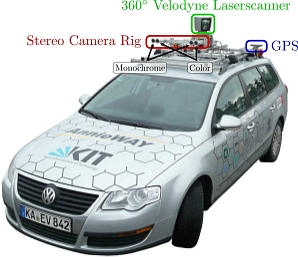
\includegraphics[width=0.3\columnwidth]{./images/kitti_sensors}
		}\hfill{}\subfloat[] 
		{
			\begin{tabular}[b]{c}%
				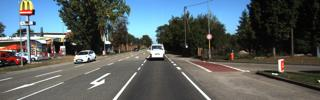
\includegraphics[width=0.3\columnwidth]{./images/kitti01}\thickspace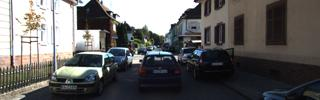
\includegraphics[width=0.3\columnwidth]{./images/kitti02}\\
				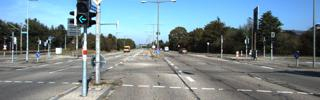
\includegraphics[width=0.3\columnwidth]{./images/kitti03}\thickspace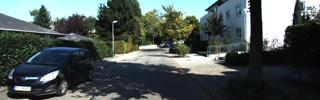
\includegraphics[width=0.3\columnwidth]{./images/kitti04}\\
				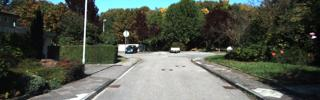
\includegraphics[width=0.3\columnwidth]{./images/kitti05}\thickspace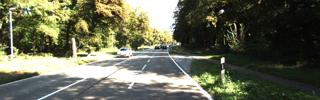
\includegraphics[width=0.3\columnwidth]{./images/kitti06}
			\end{tabular}
		}\\
		\subfloat[] 
		{
			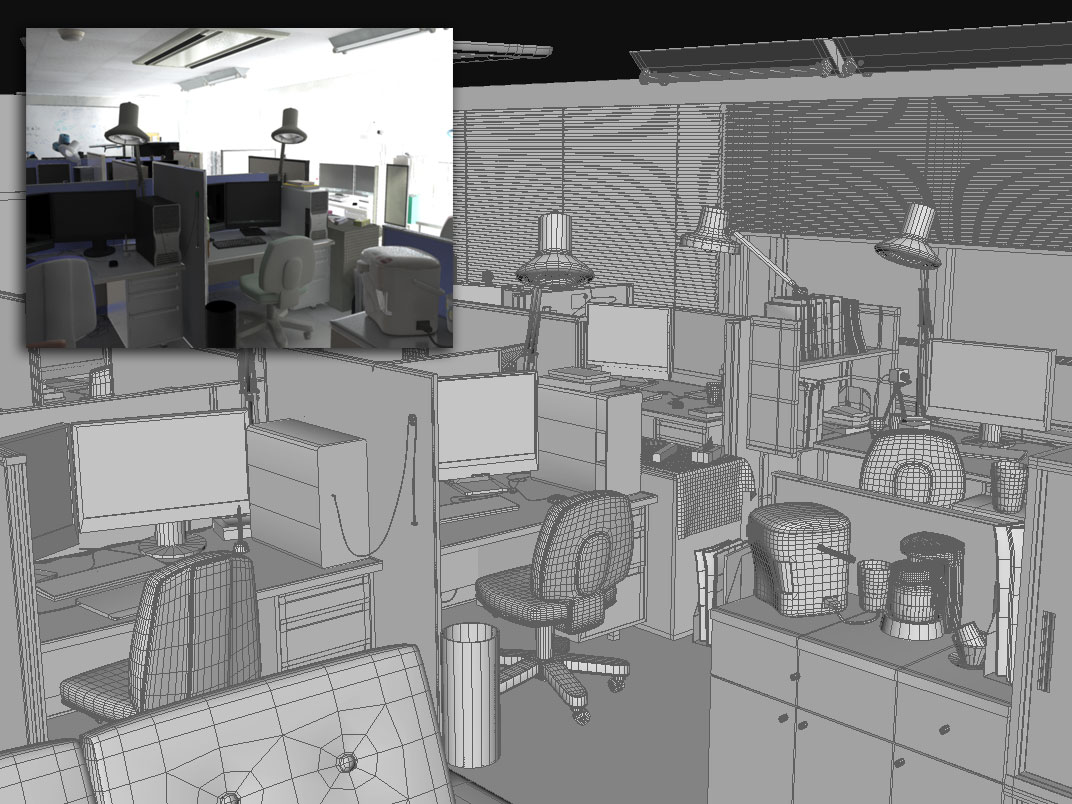
\includegraphics[width=0.3\columnwidth]{./images/tsukuba_dataset}
		}\hspace{0.2cm}\subfloat[] 
		{
			\begin{tabular}[b]{c}%
				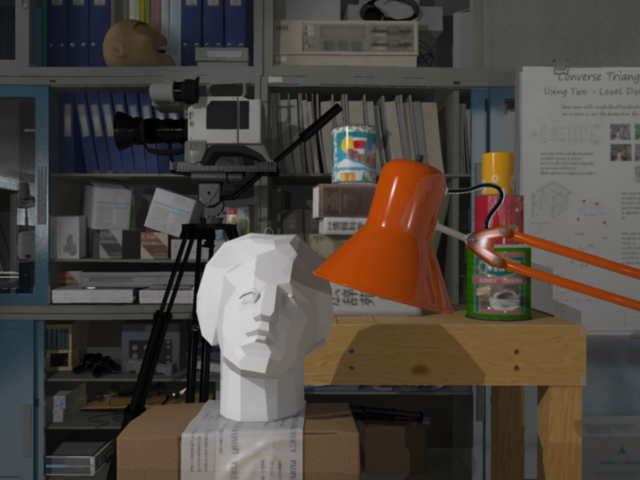
\includegraphics[width=0.2\columnwidth]{./images/tsukuba_sample1}\thickspace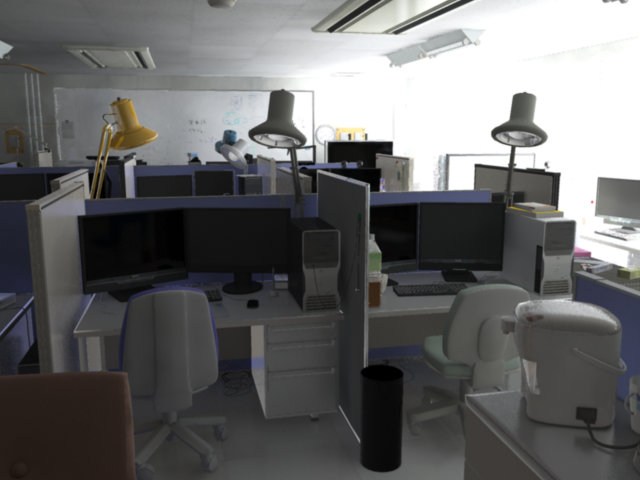
\includegraphics[width=0.2\columnwidth]{./images/tsukuba_sample2}\\
				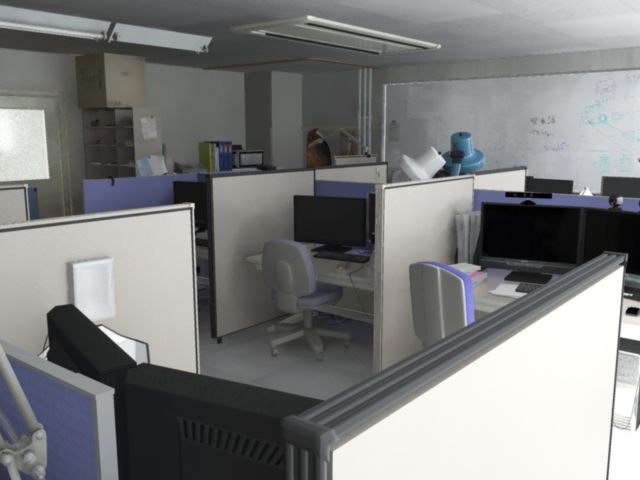
\includegraphics[width=0.2\columnwidth]{./images/tsukuba_sample3}\thickspace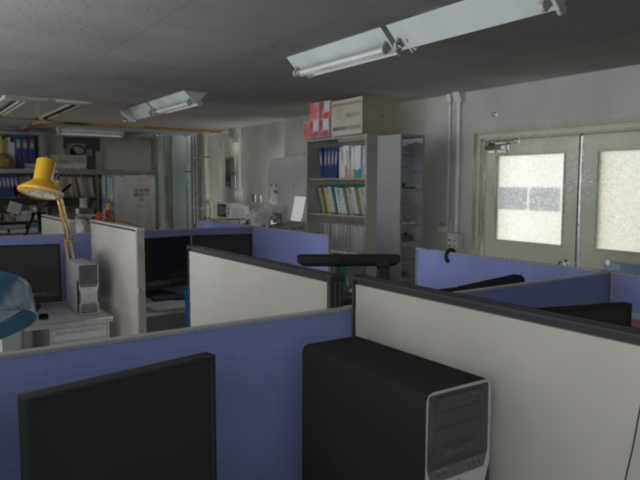
\includegraphics[width=0.2\columnwidth]{./images/tsukuba_sample4}				
			\end{tabular}
		}
	\end{figure}
\end{frame}


\begin{frame}
	\frametitle{KITTI: Reconstrucción 3D}
\begin{figure}[!htb]
	\centering
	{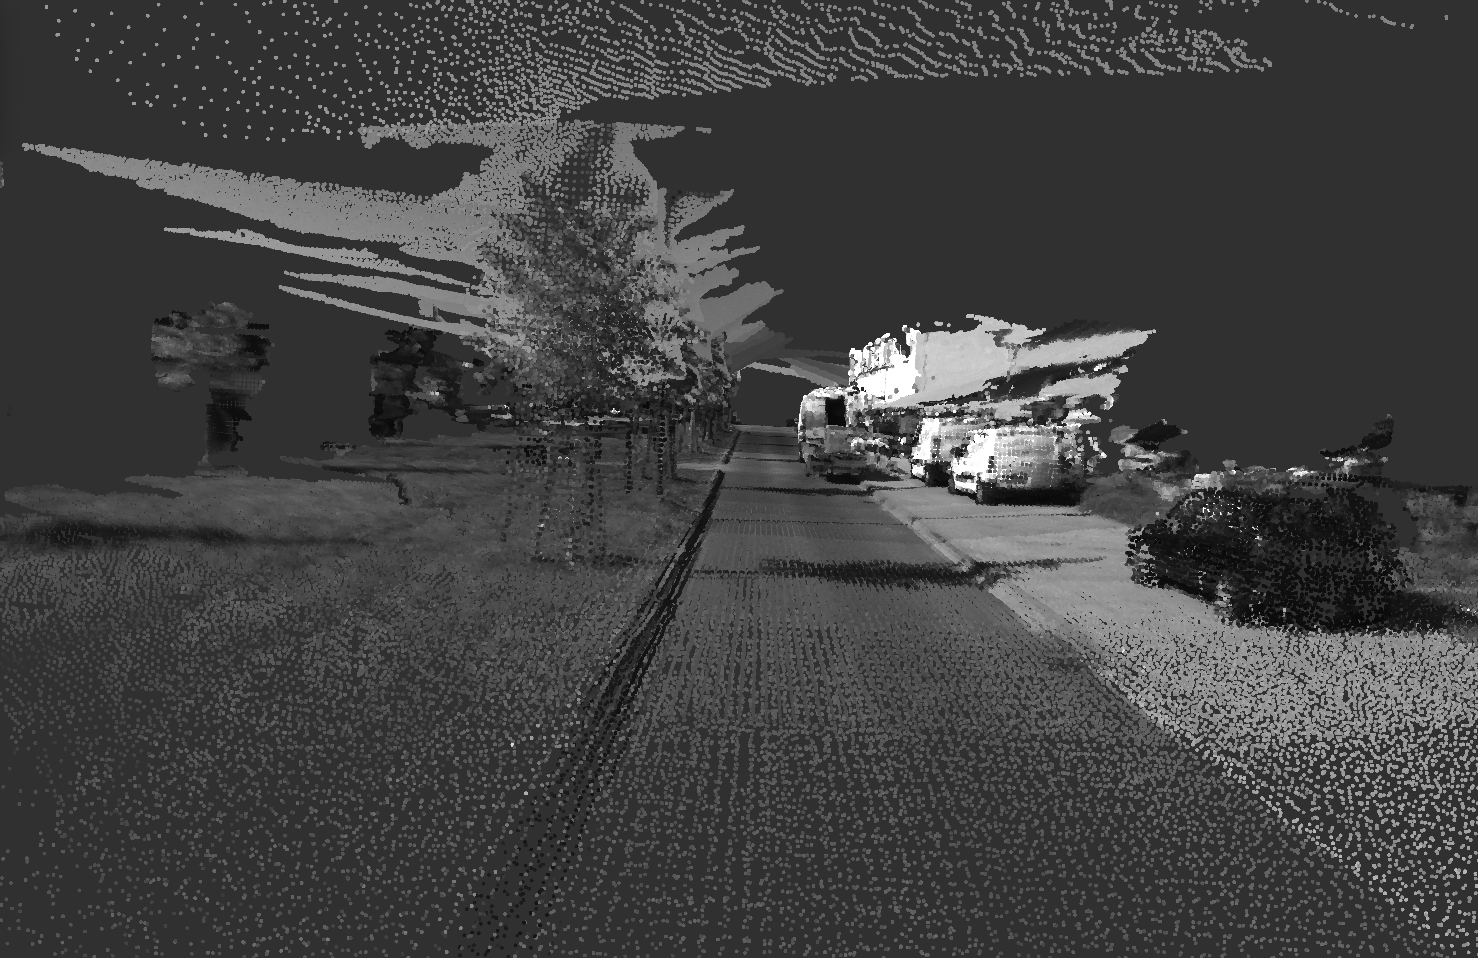
\includegraphics[width=0.32\columnwidth]{./images/kitti_3d_1}%
		\label{kitti_3d_1}}
	\hfil
	{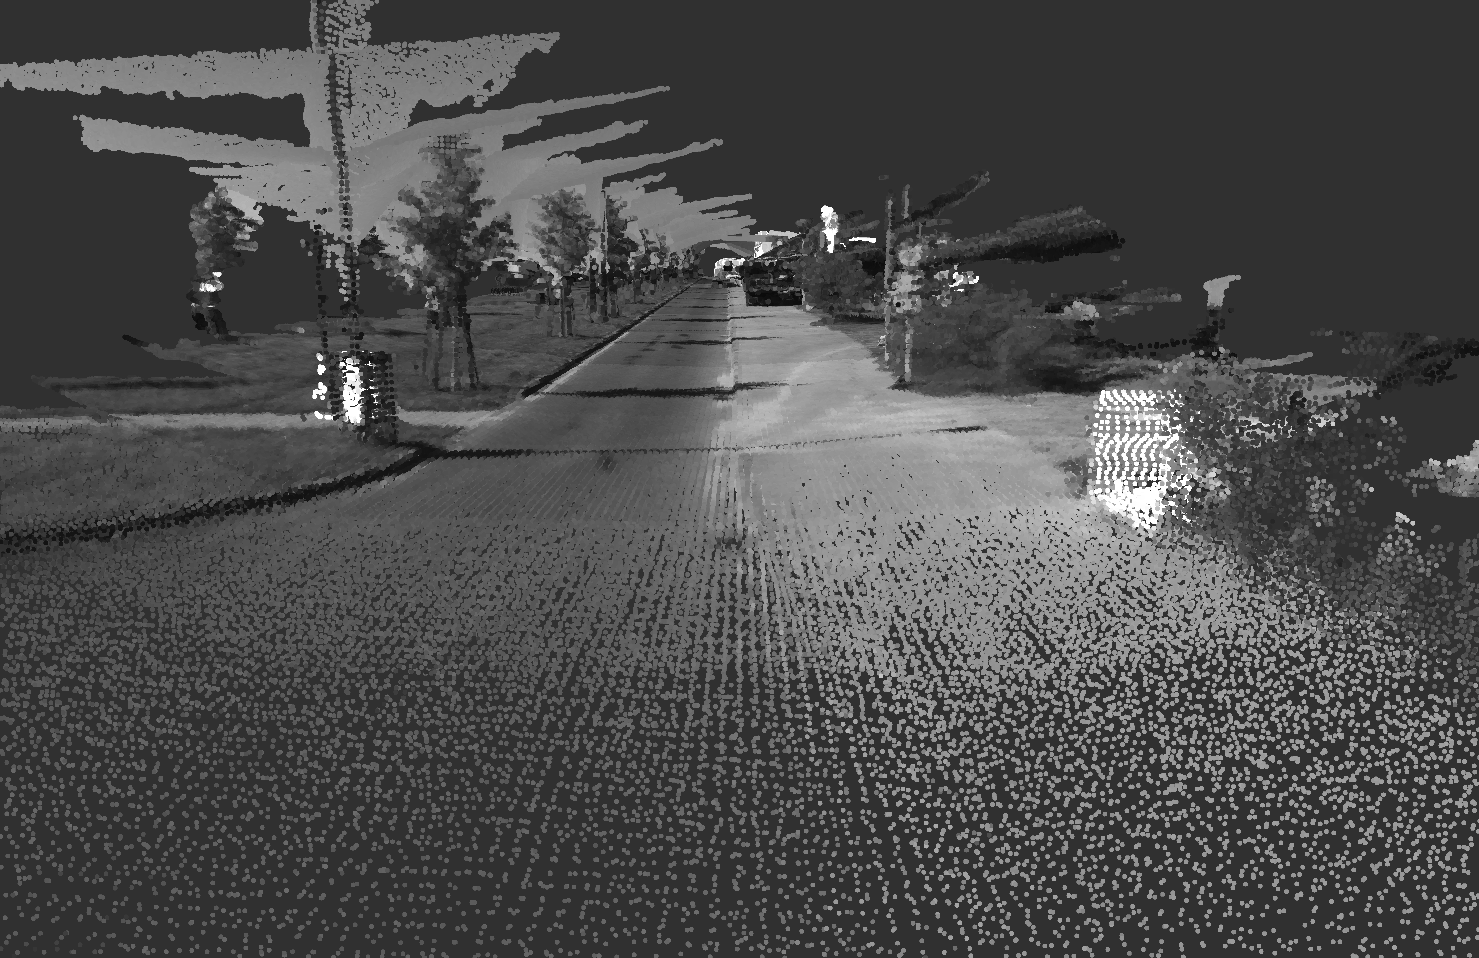
\includegraphics[width=0.32\columnwidth]{./images/kitti_3d_2}%
		\label{kitti_3d_2}}
	\hfil
	{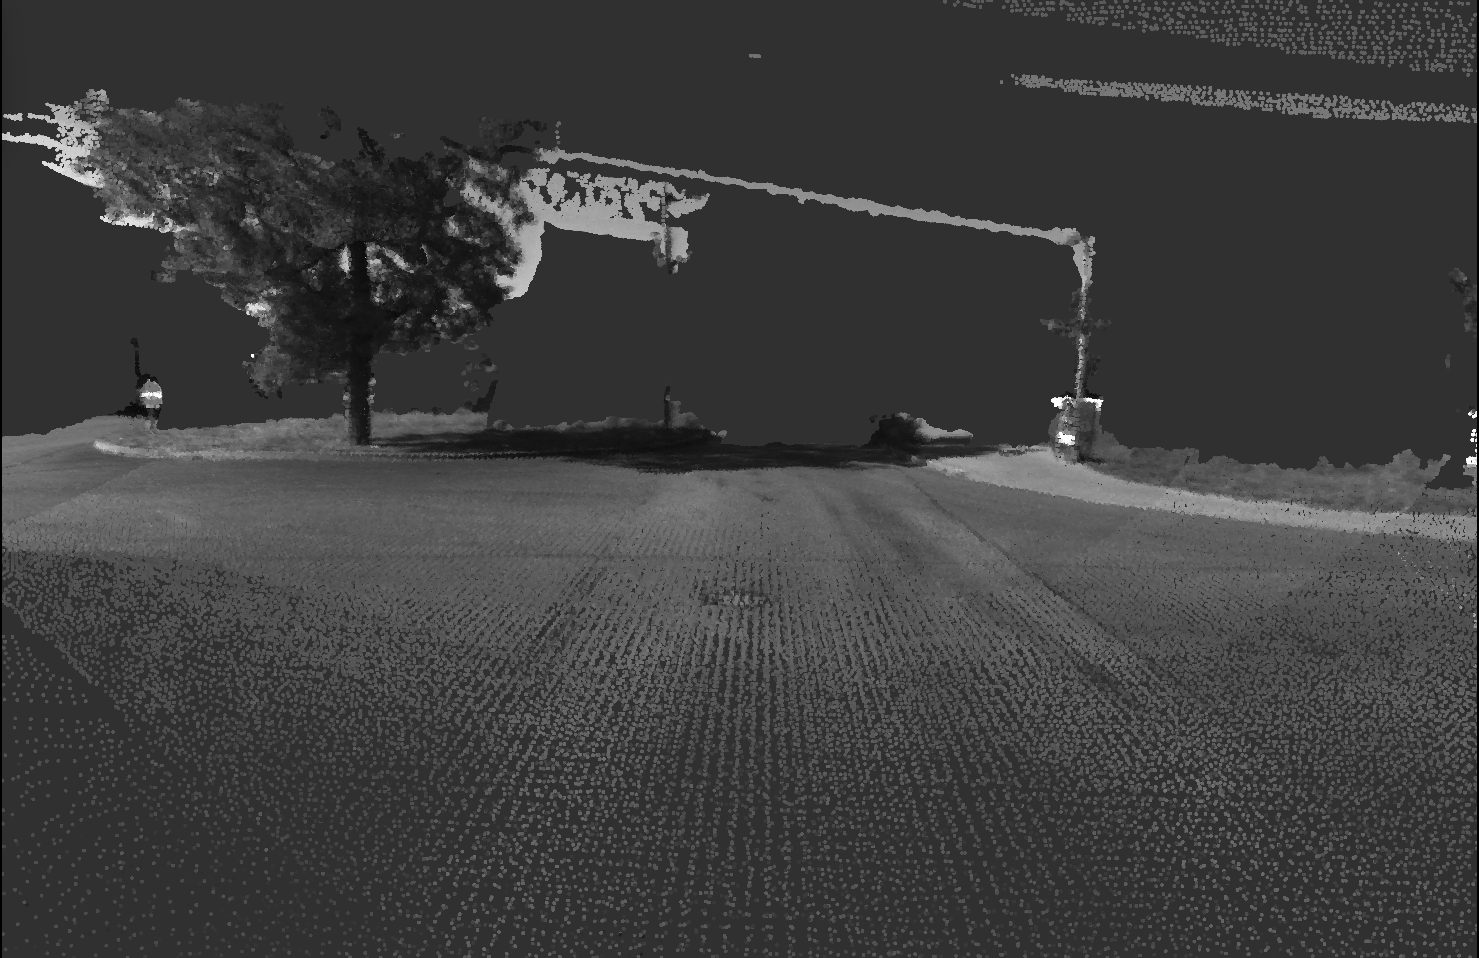
\includegraphics[width=0.32\columnwidth]{./images/kitti_3d_3}%
		\label{kitti_3d_3}}
	\caption{Vistas de la reconstrucción 3D obtenidas para el dataset KITTI.}
	\label{fig:kitti_reconstructions}
\end{figure}
\end{frame}

\begin{frame}
	\frametitle{Tsukuba: Reconstrucción 3D}
\begin{figure}[!htb]
	\centering
	{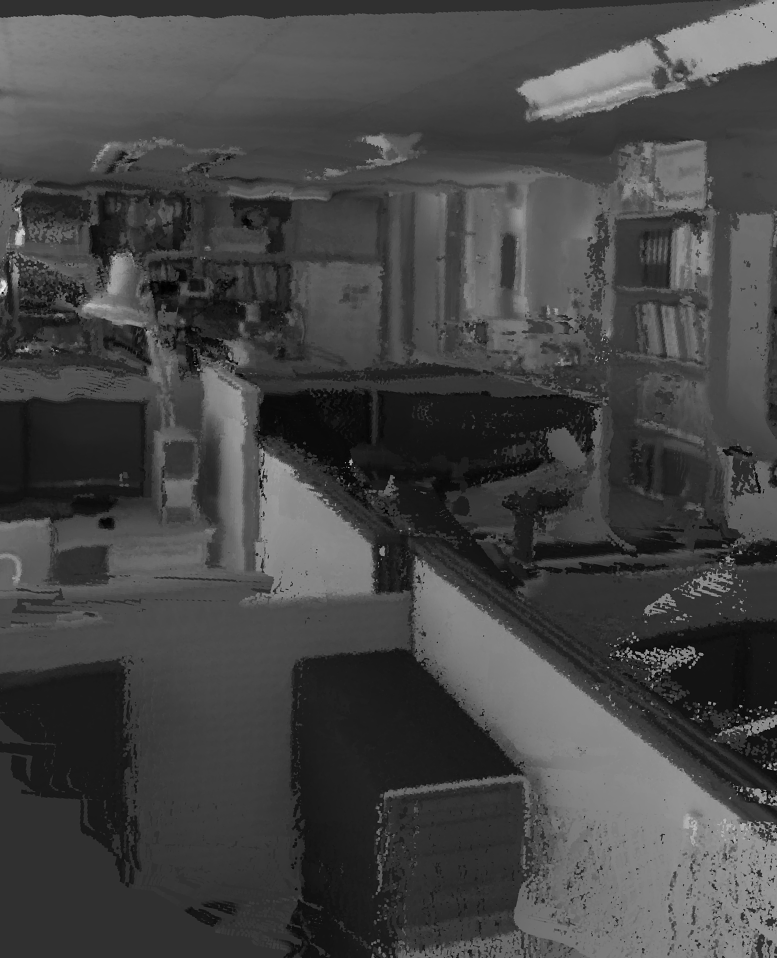
\includegraphics[width=0.32\columnwidth, height=3.5cm]{./images/tsukuba_3d_1}%
		\label{tsukuba_3d_1}}
	\hfil
	{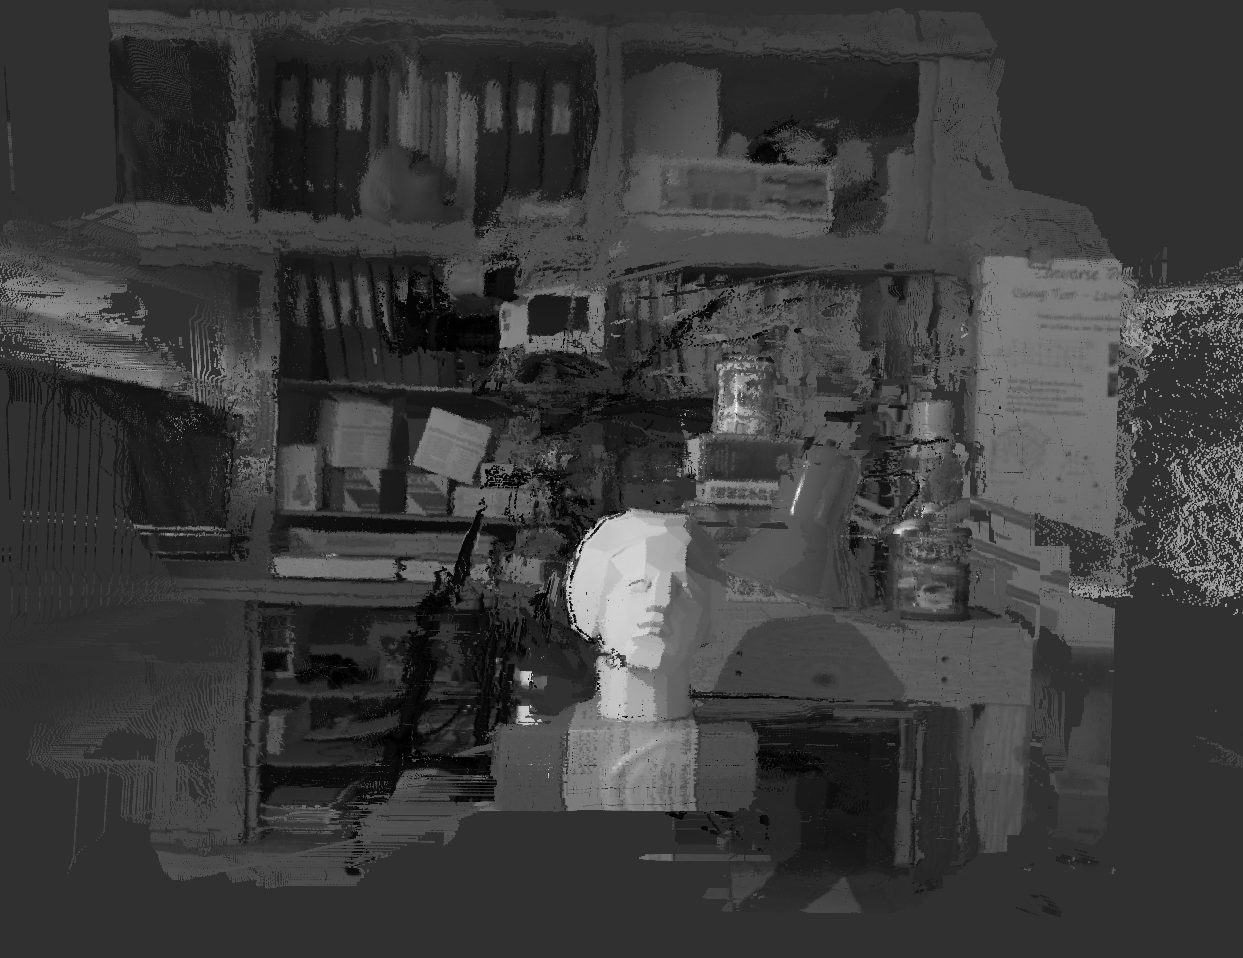
\includegraphics[width=0.32\columnwidth, height=3.5cm]{./images/tsukuba_3d_2}%
		\label{tsukuba_3d_2}}
	\hfil
	{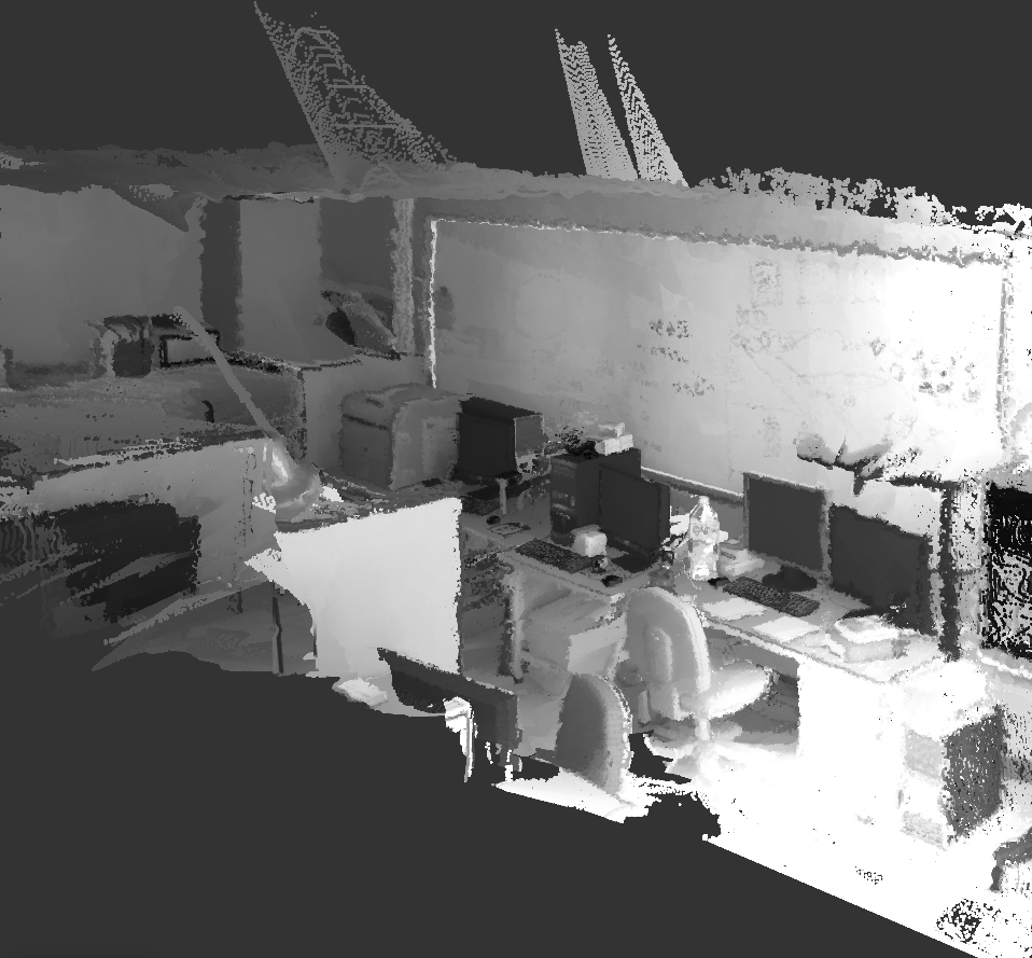
\includegraphics[width=0.32\columnwidth, height=3.5cm]{./images/tsukuba_3d_3}%
		\label{tsukuba_3d_3}}
	
	\caption{Vistas de la reconstrucción 3D obtenidas para el dataset Tsukuba.}
	\label{fig:tsukuba_reconstructions}
\end{figure}
\end{frame}

\begin{frame}
	\frametitle{KITTI: error de reconstrucción}
\begin{figure}[!htb]
	\centering
	\subfloat[Left image]{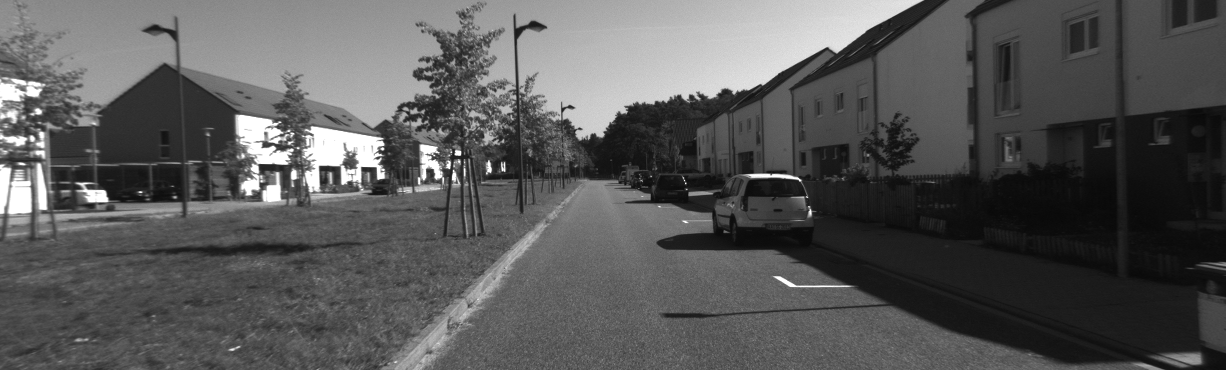
\includegraphics[width=0.45\columnwidth]{./images/kitti06_frame612_rgb.png}%
		\label{kitti06_frame612_rgb}}
	\hfil
	\subfloat[Ground-Truth]{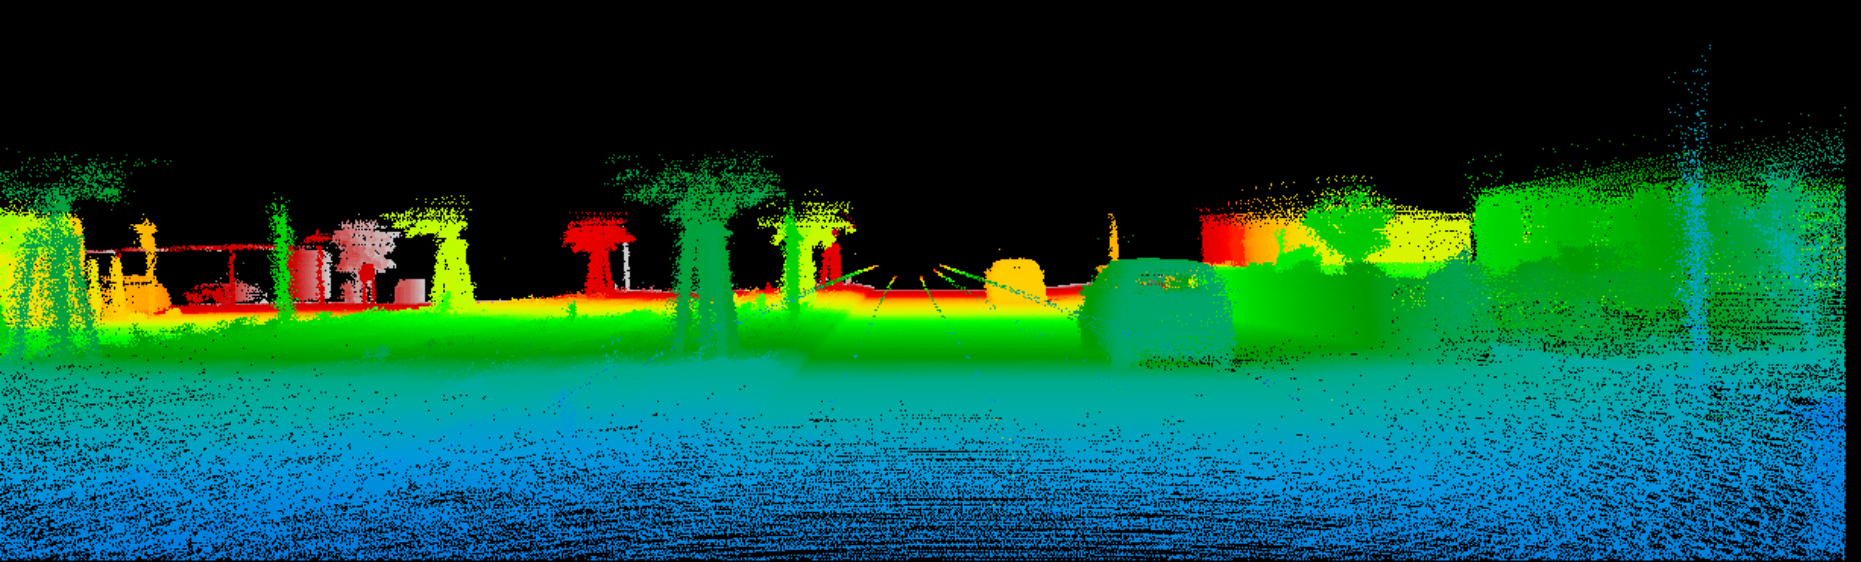
\includegraphics[width=0.45\columnwidth]{./images/kitti06_frame612_gt_high50.png}%
		\label{kitti06_frame612_gt}}
	\\
	\subfloat[LIBELAS depth map]{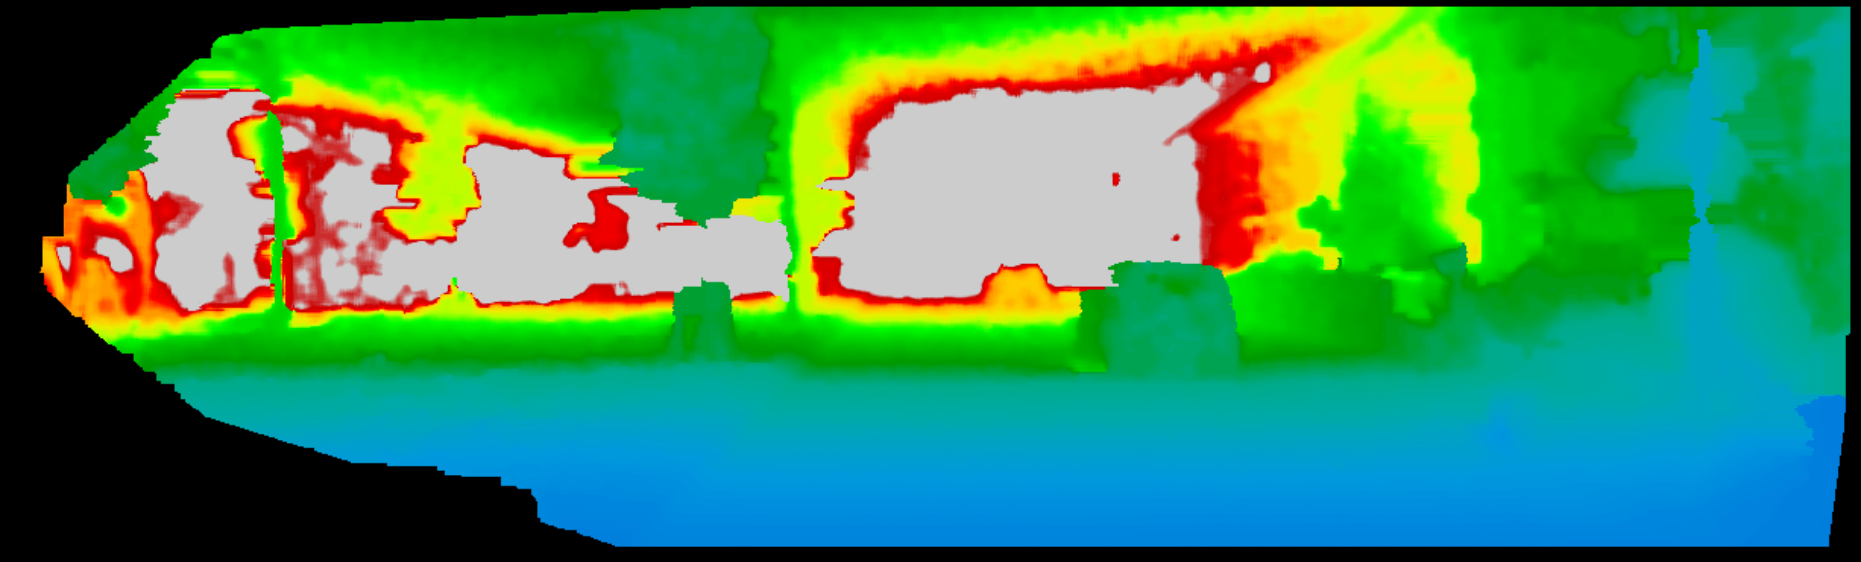
\includegraphics[width=0.45\columnwidth]{./images/kitti06_frame612_libelas_depth_high50.png}%
		\label{kitti06_frame612_libelas_depth}}
	\hfil
	\subfloat[LIBELAS depth map error]{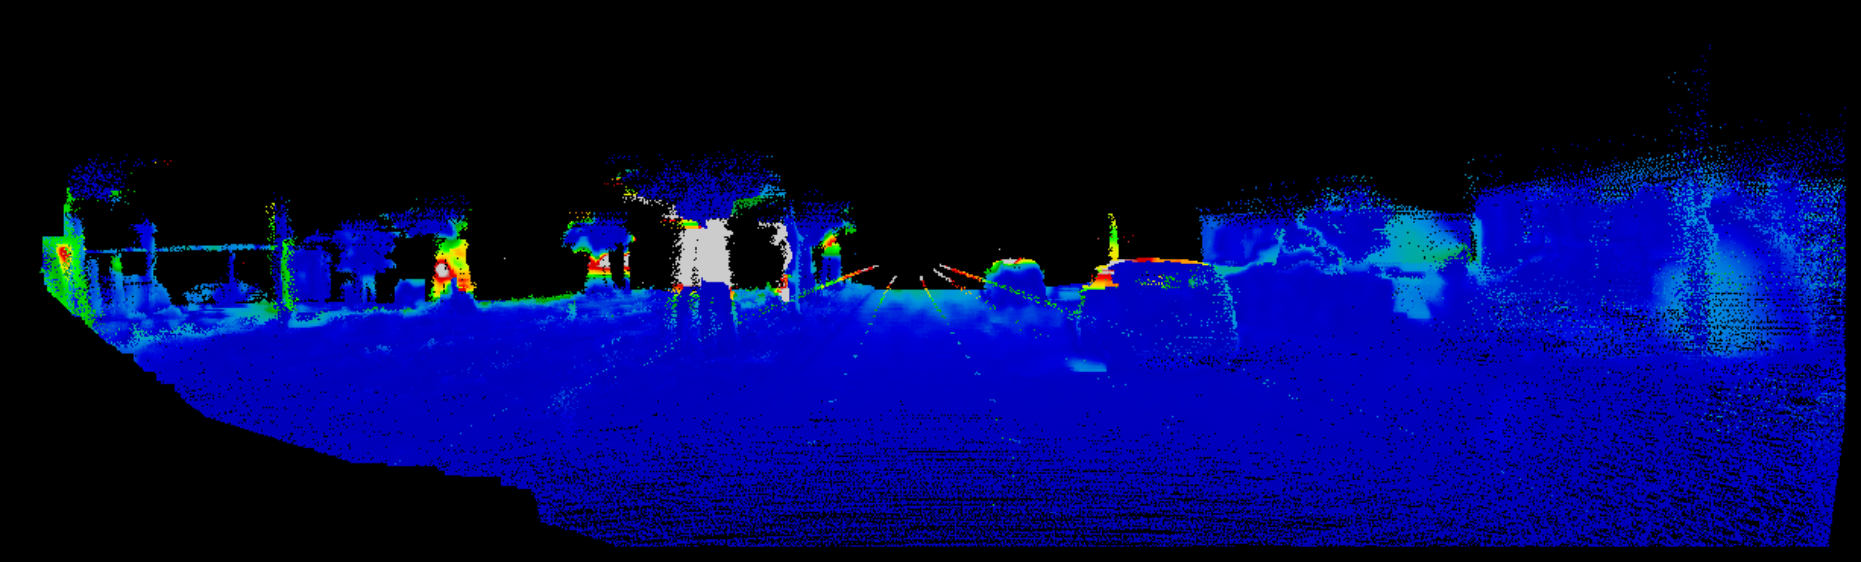
\includegraphics[width=0.45\columnwidth]{./images/kitti06_frame612_libelas_error_high50.png}%
		\label{kitti06_frame612_libelas_error}}
	\\
	\subfloat[Dense S-PTAM depth map]{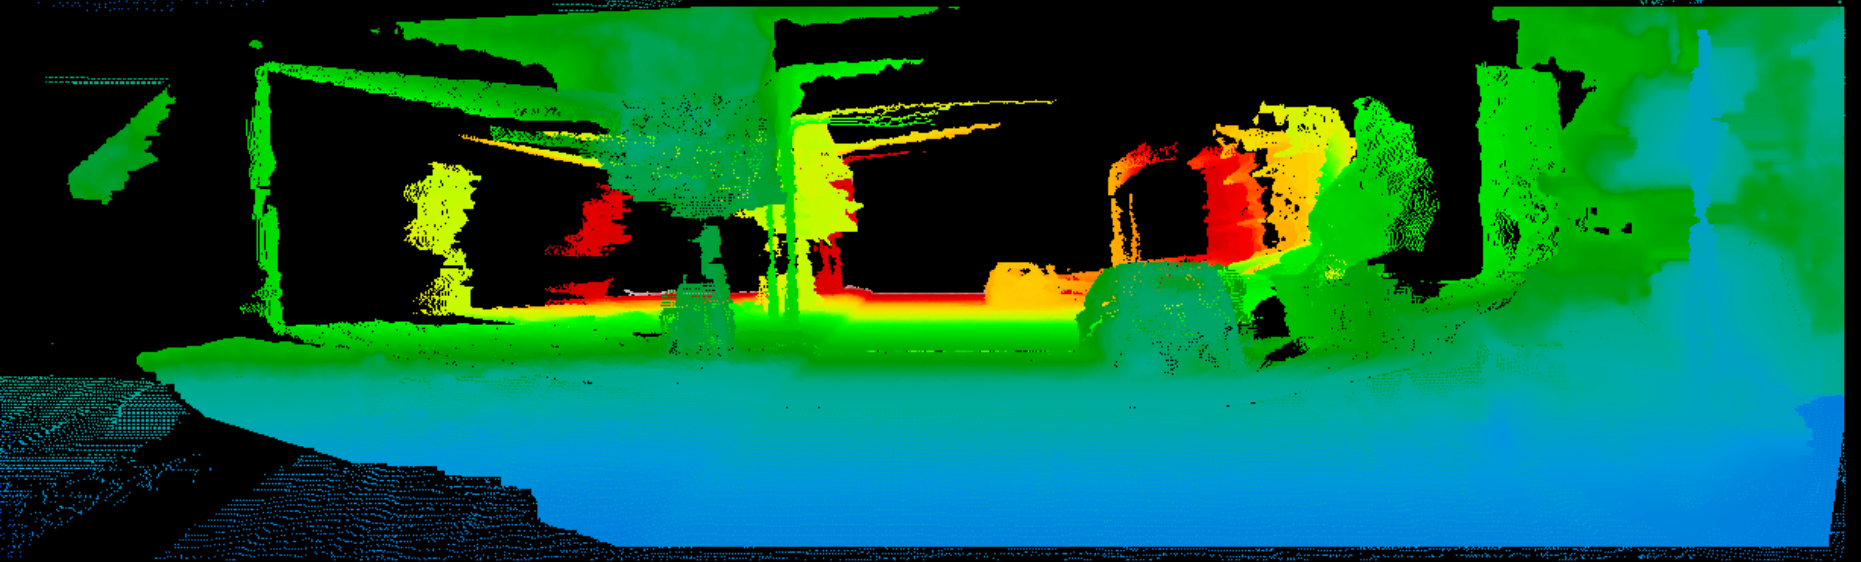
\includegraphics[width=0.45\columnwidth]{./images/kitti06_frame612_dense_high50.png}%
		\label{kitti06_frame612_dense}}
	\hfil
	\subfloat[Dense S-PTAM depth map error]{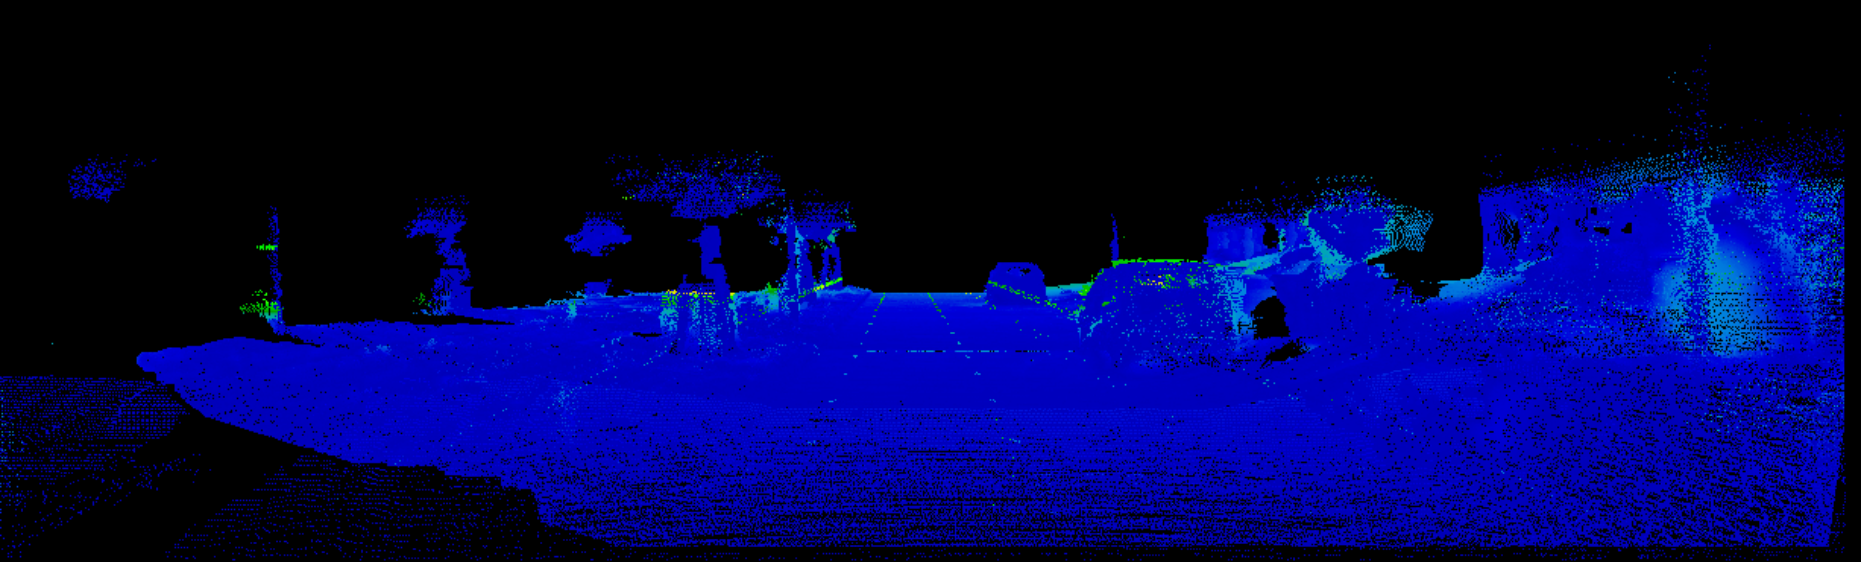
\includegraphics[width=0.45\columnwidth]{./images/kitti06_frame612_error_high50.png}%
		\label{kitti06_frame612_error}}
	\\
	\subfloat[Color metric]{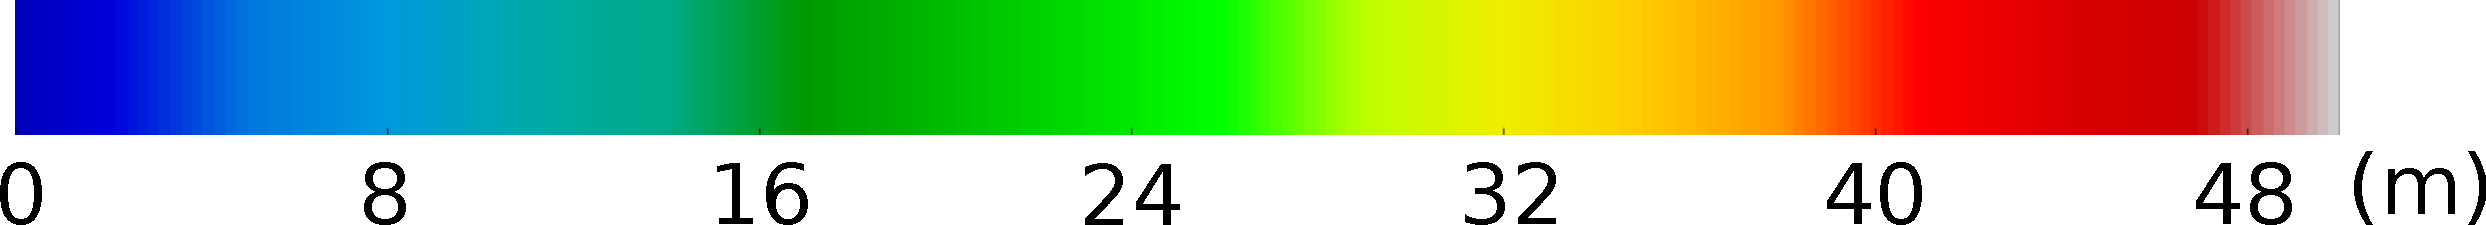
\includegraphics[width=0.45\columnwidth]{./images/high50_bar.pdf}%
		\label{kitti06_bar}}
	%\caption{Comparison of LIBELAS and Dense S-PTAM depth maps against the ground truth, for a single frame (KITTI dataset).}
	\label{fig:kitti06_frame612}
\end{figure}
\end{frame}

%\begin{frame}
%	\frametitle{KITTI: error de reconstrucción}
%\begin{figure}[!htb]
%	\centering
%	\subfloat[Left image]{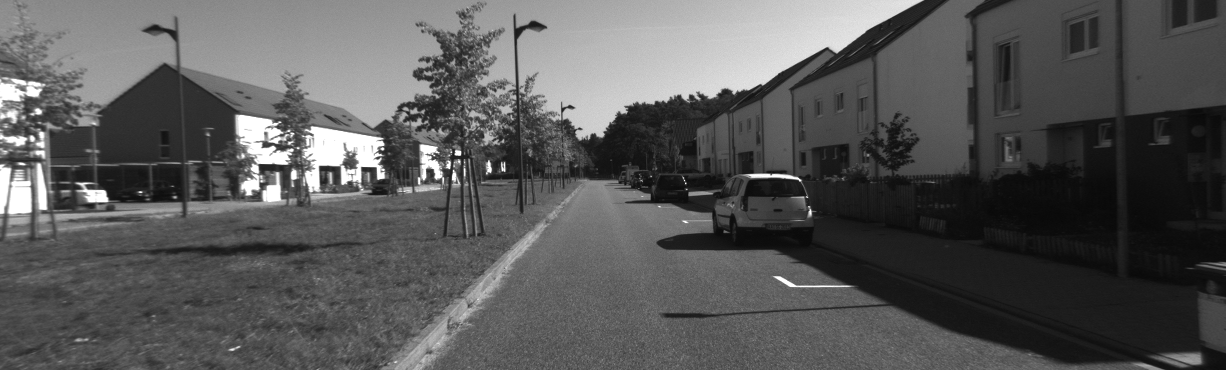
\includegraphics[width=0.45\columnwidth]{./images/kitti06_frame612_rgb.png}%
%		\label{kitti06_frame777_rgb}}
%	\hfil
%	\subfloat[Ground-Truth]{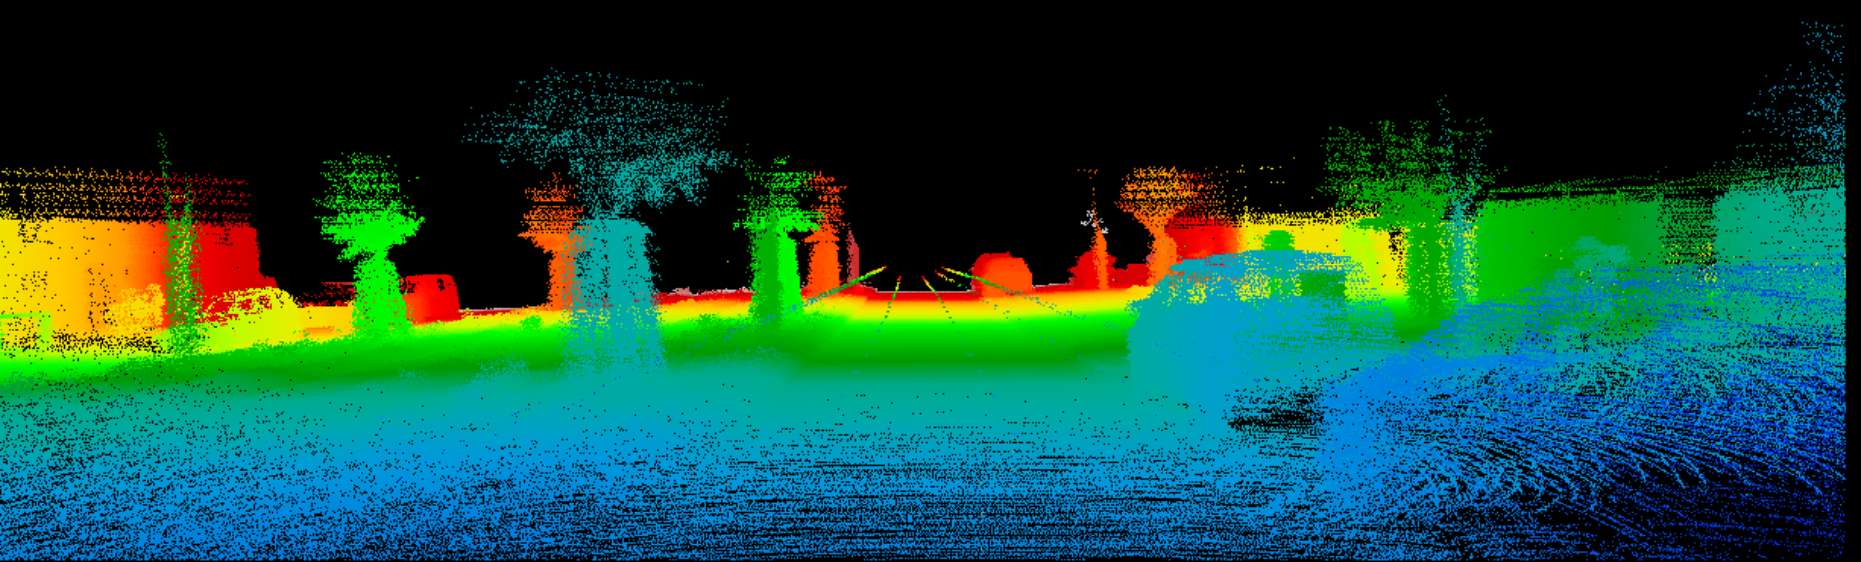
\includegraphics[width=0.45\columnwidth]{./images/kitti06_frame777_gt_high50.png}%
%		\label{kitti06_frame777_gt}}
%	\\
%	\subfloat[LIBELAS depth map]{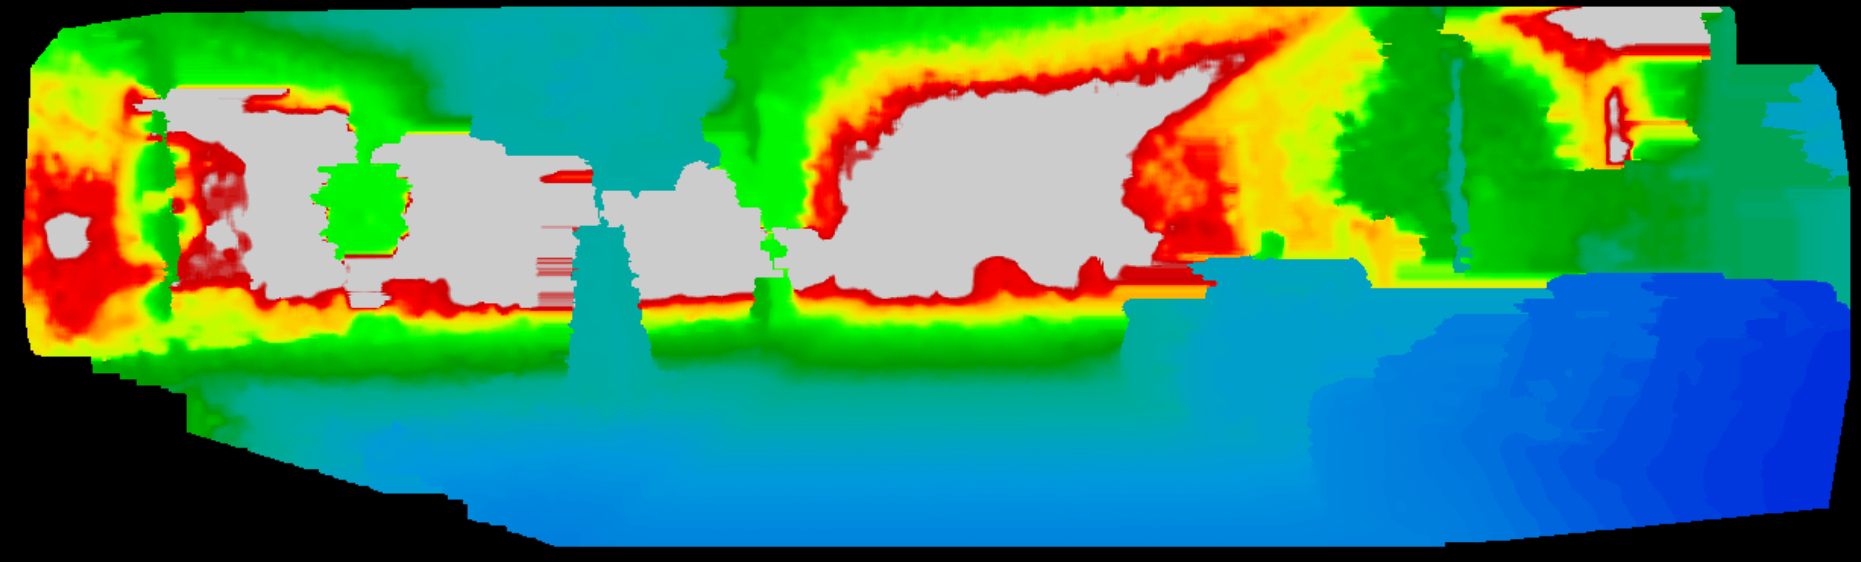
\includegraphics[width=0.45\columnwidth]{./images/kitti06_frame777_libelas_depth_high50.png}%
%		\label{kitti06_frame777_libelas_depth}}
%	\hfil
%	\subfloat[LIBELAS Depth map error]{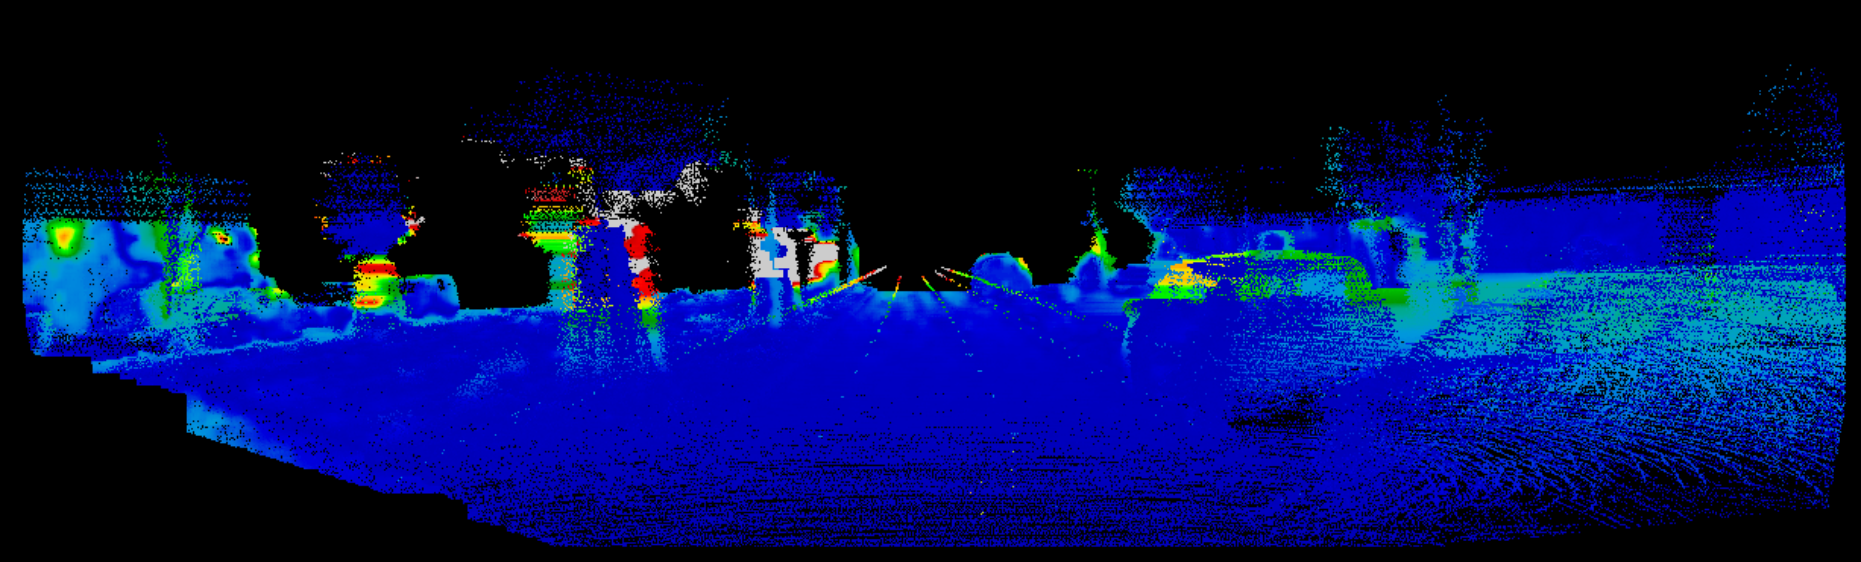
\includegraphics[width=0.45\columnwidth]{./images/kitti06_frame777_libelas_error_high50.png}%
%		\label{kitti06_frame777_libelas_error}}
%	\\
%	\subfloat[Dense S-PTAM depth map]{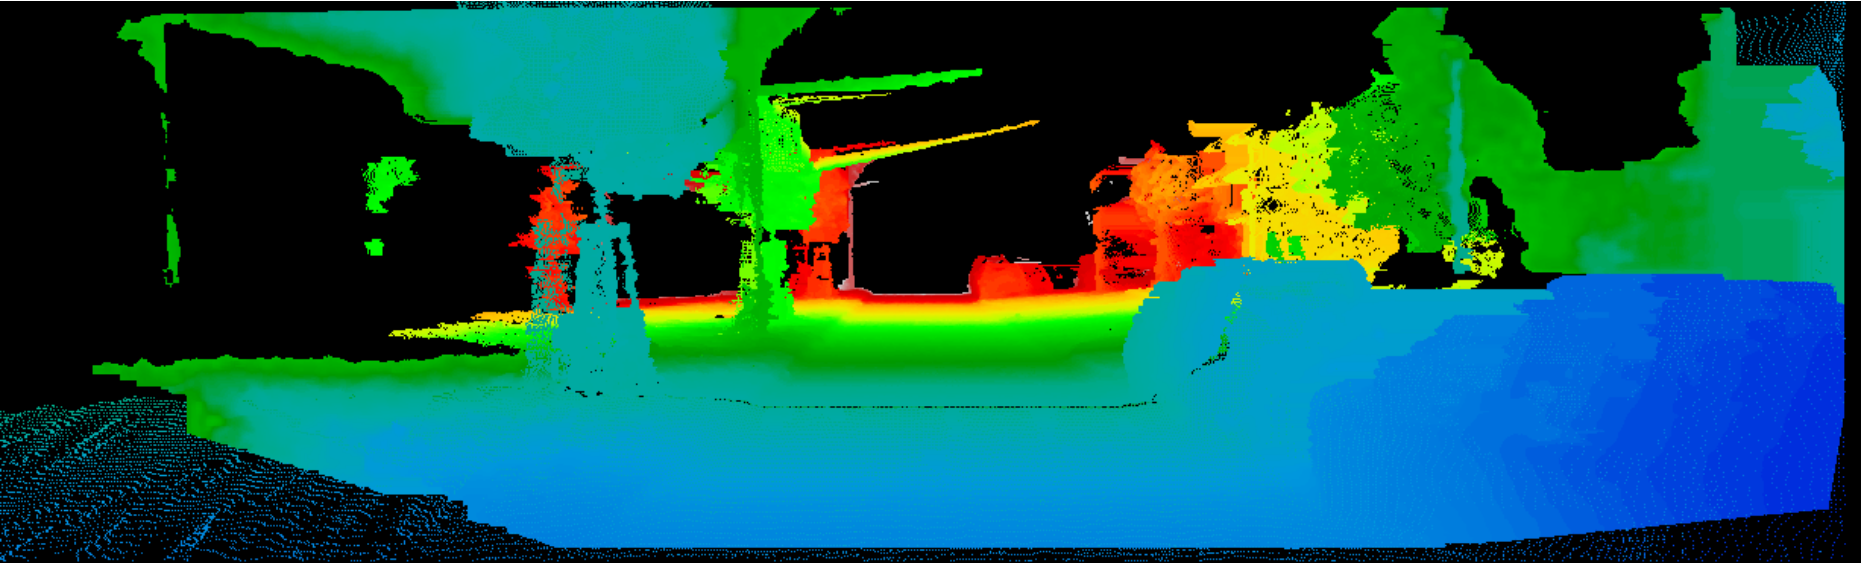
\includegraphics[width=0.45\columnwidth]{./images/kitti06_frame777_dense_high50.png}%
%		\label{kitti06_frame777_dense}}
%	\hfil
%	\subfloat[Dense S-PTAM depth map error]{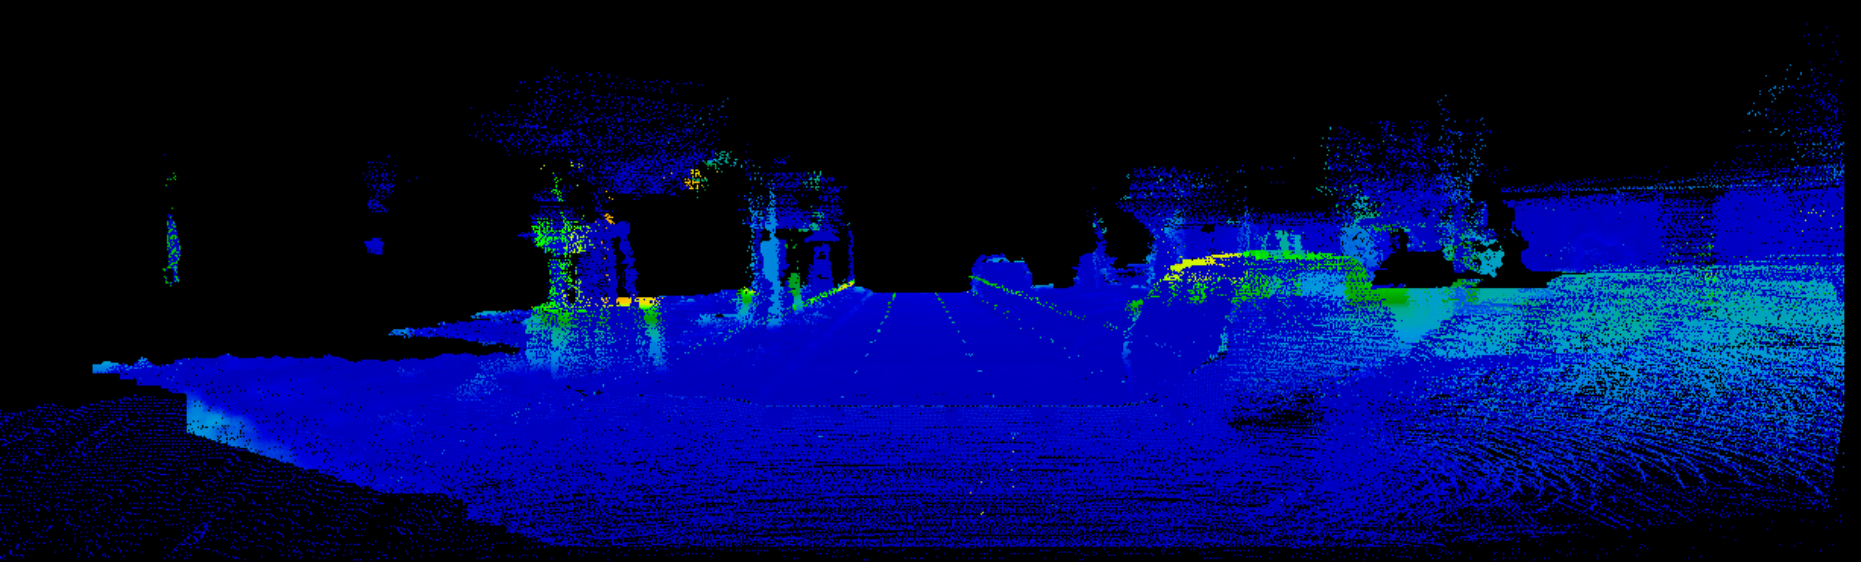
\includegraphics[width=0.45\columnwidth]{./images/kitti06_frame777_error_high50.png}%
%		\label{kitti06_frame777_error}}
%	\\
%	\subfloat[Color metric]{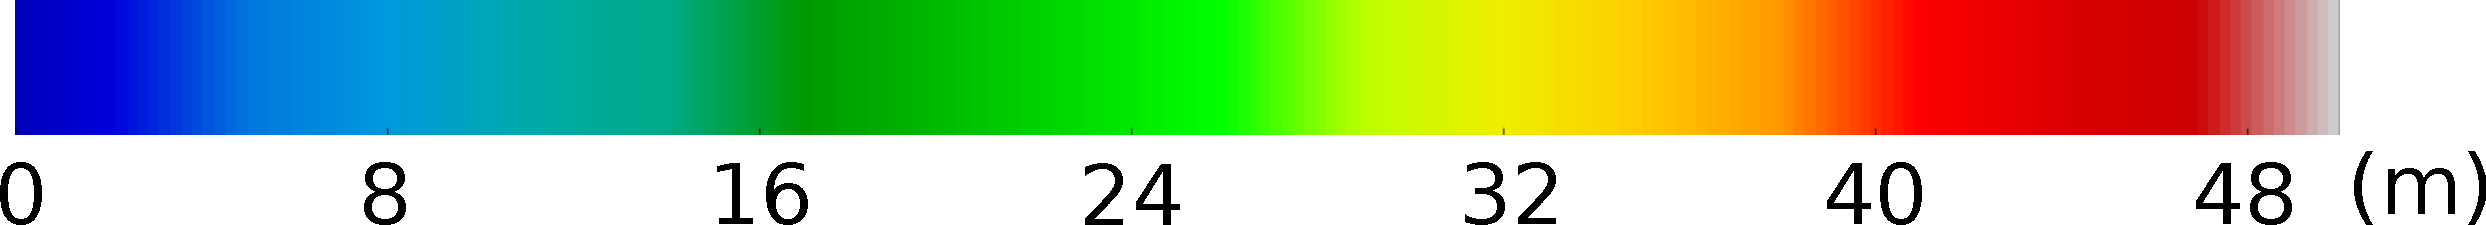
\includegraphics[width=0.45\columnwidth]{./images/high50_bar.pdf}%
%		\label{kitti06_frame777_bar}}
%	\caption{Comparison of LIBELAS and Dense S-PTAM depth maps against the ground truth, for a single frame (KITTI dataset).}
%	\label{fig:kitti06_frame777}
%\end{figure}
%\end{frame}


\begin{frame}
	\frametitle{Tsukuba: error de reconstrucción}
% tsukuba
\begin{figure}[!htb]
	\centering
	\subfloat[Left image]{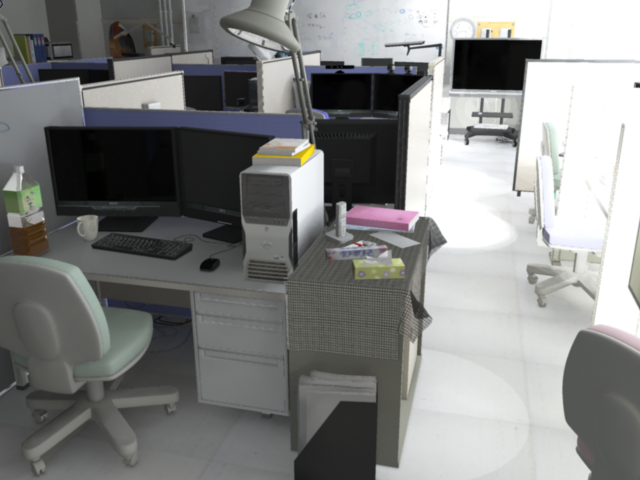
\includegraphics[width=0.2\columnwidth]{./images/tsukuba_frame807_rgb.png}%
		\label{tsukuba_frame807_rgb}}
	\hfil
	\subfloat[Ground Truth]{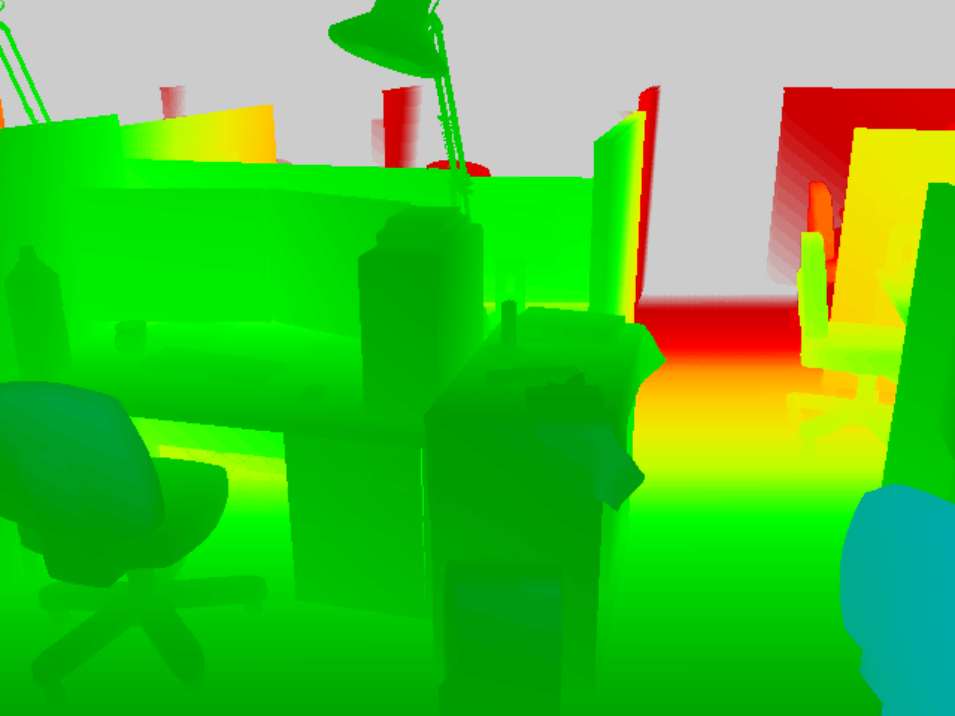
\includegraphics[width=0.2\columnwidth]{./images/tsukuba_frame807_gt_high6.png}%
		\label{tsukuba_gt}}
    \\
	\subfloat[LIBELAS dmap]{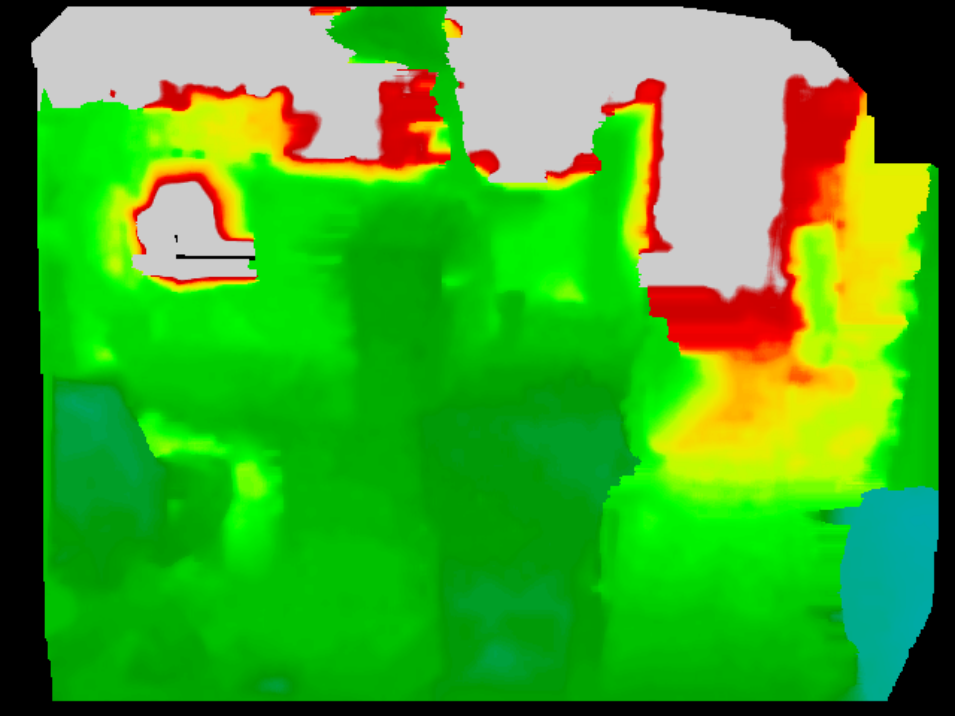
\includegraphics[width=0.2\columnwidth]{./images/tsukuba_frame807_libelas_depth_high6.png}%
		\label{tsukuba_frame807_libelas_depth}}
	\hfil
	\subfloat[LIBELAS dmap error]{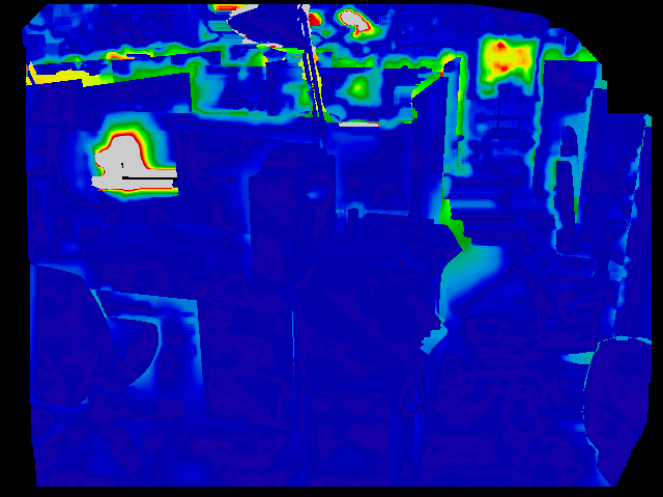
\includegraphics[width=0.2\columnwidth]{./images/tsukuba_frame807_libelas_error_high6.png}%
		\label{tsukuba_frame807_libelas_error}}
    \hfil
	\subfloat[Dense S-PTAM dmap]{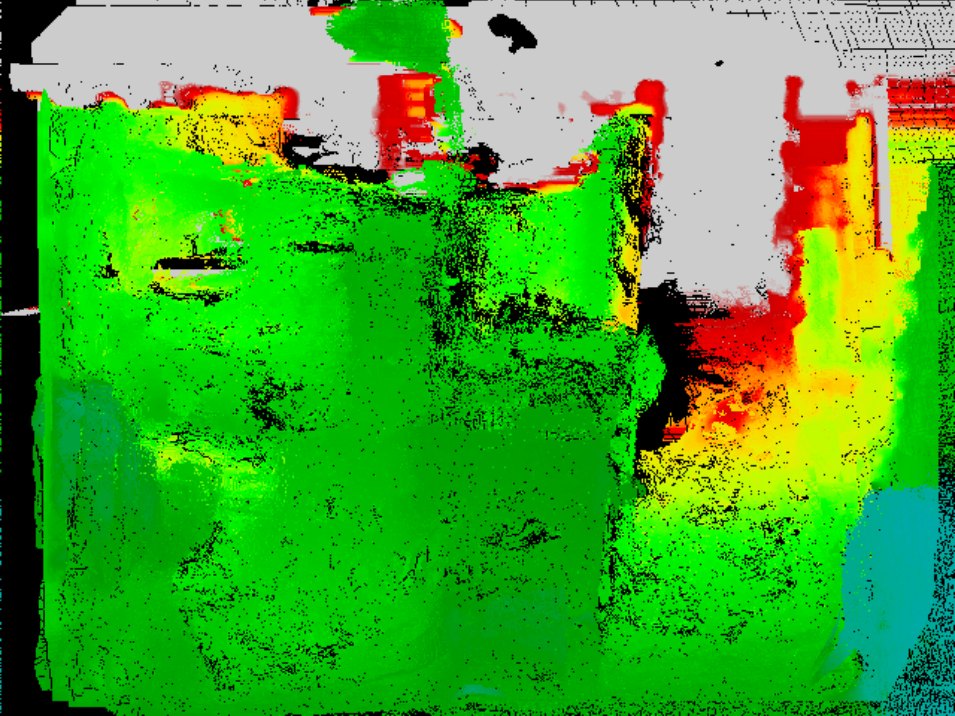
\includegraphics[width=0.2\columnwidth]{./images/tsukuba_frame807_dense_high6.png}%
		\label{tsukuba_frame807_dense}}
	\hfil
	\subfloat[Dense S-PTAM dmap error]{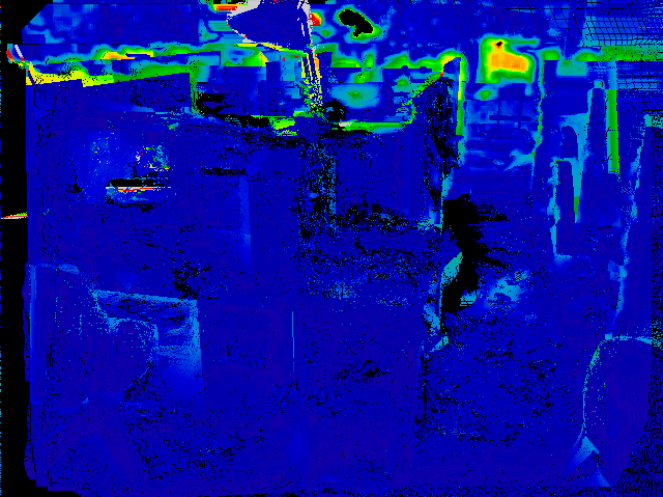
\includegraphics[width=0.2\columnwidth]{./images/tsukuba_frame807_error_high6.png}%
		\label{tsukuba_frame807_error}}
	\\
	\subfloat[]{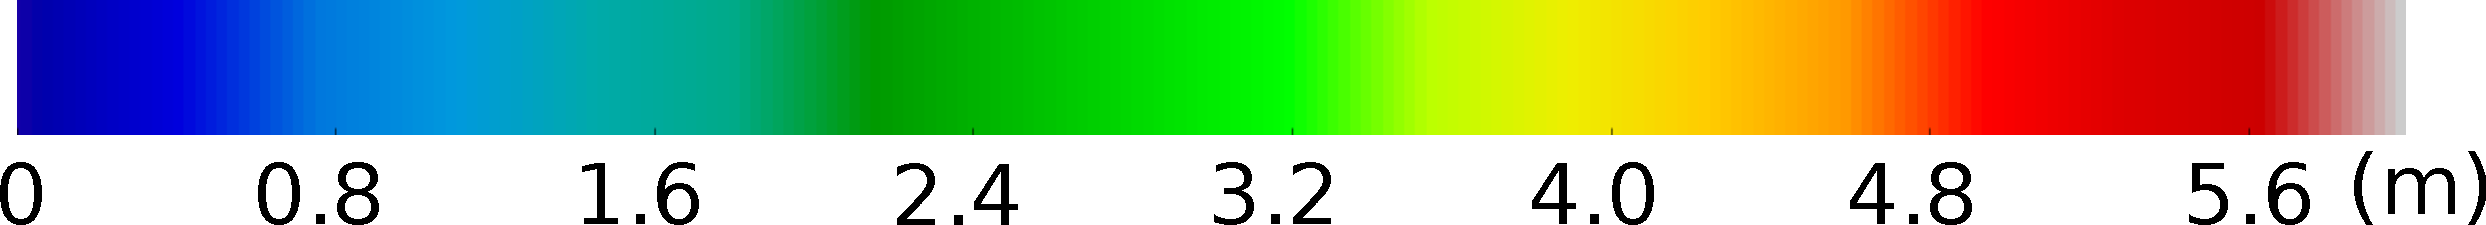
\includegraphics[width=0.4\columnwidth]{./images/high6_bar.pdf}%
		\label{tsukuba_frame807_bar}}
	%\caption{Comparison: LIBELAS, DS-PTAM dmaps against GT (Tsukuba).}
	\label{fig:tsukuba_frame807}
\end{figure}
\end{frame}

%\begin{frame}
%	\frametitle{Tsukuba: error de reconstrucción}
%	\begin{figure}[!htb]
%		\centering
%		\subfloat[Left image]{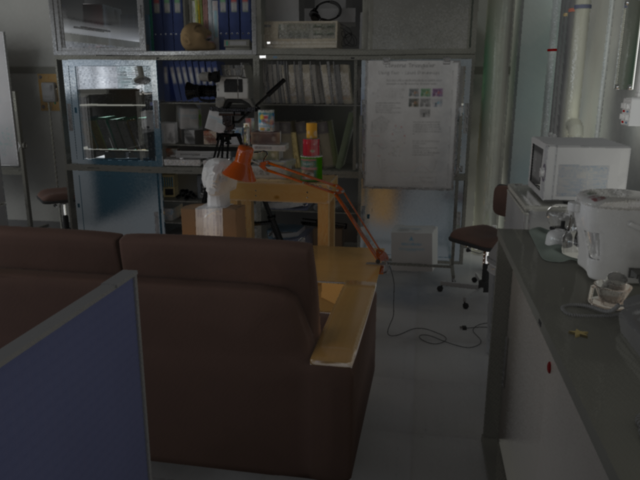
\includegraphics[width=0.2\columnwidth]{./images/tsukuba_frame1314_rgb.png}%
%			\label{tsukuba_frame1314_rgb}}
%        \hfil
%		\subfloat[Ground Truth]{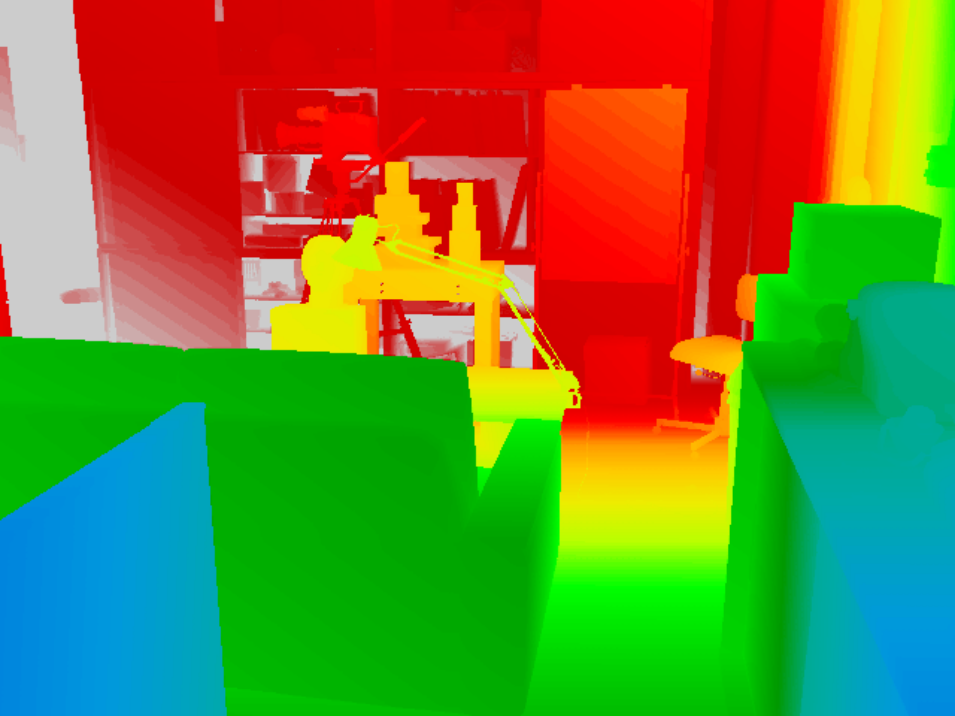
\includegraphics[width=0.2\columnwidth]{./images/tsukuba_frame1314_gt_high6.png}%
%			\label{tsukuba_frame1314_gt}}
%        \\
%		\subfloat[LIBELAS dmap]{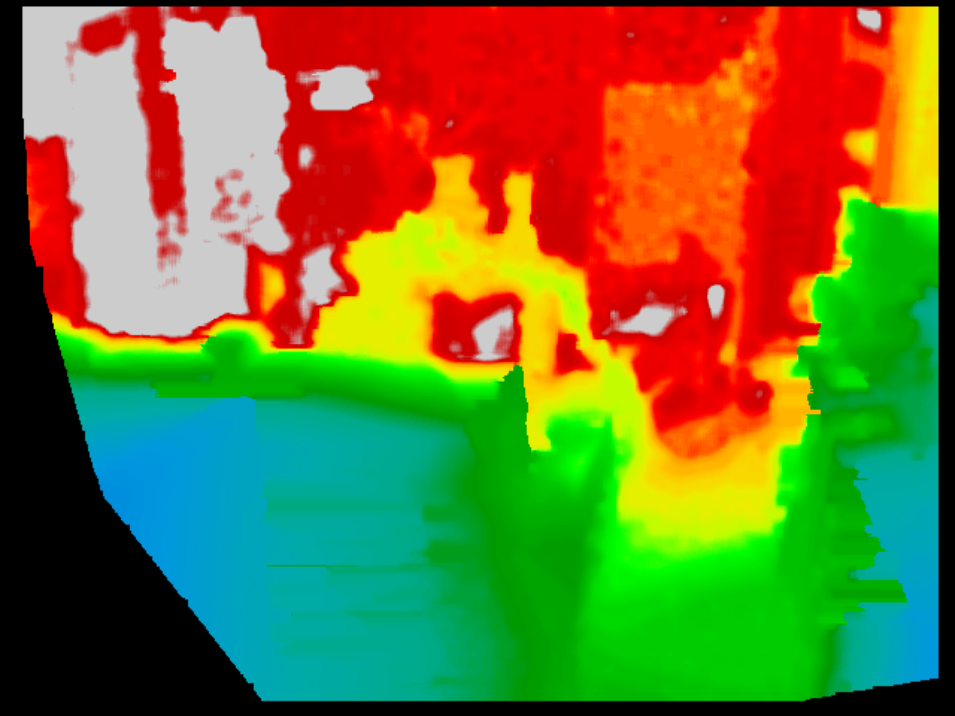
\includegraphics[width=0.2\columnwidth]{./images/tsukuba_frame1314_libelas_depth_high6.png}%
%			\label{tsukuba_frame1314_libelas_depth}}
%        \hfil
%		\subfloat[LIBELAS dmap error]{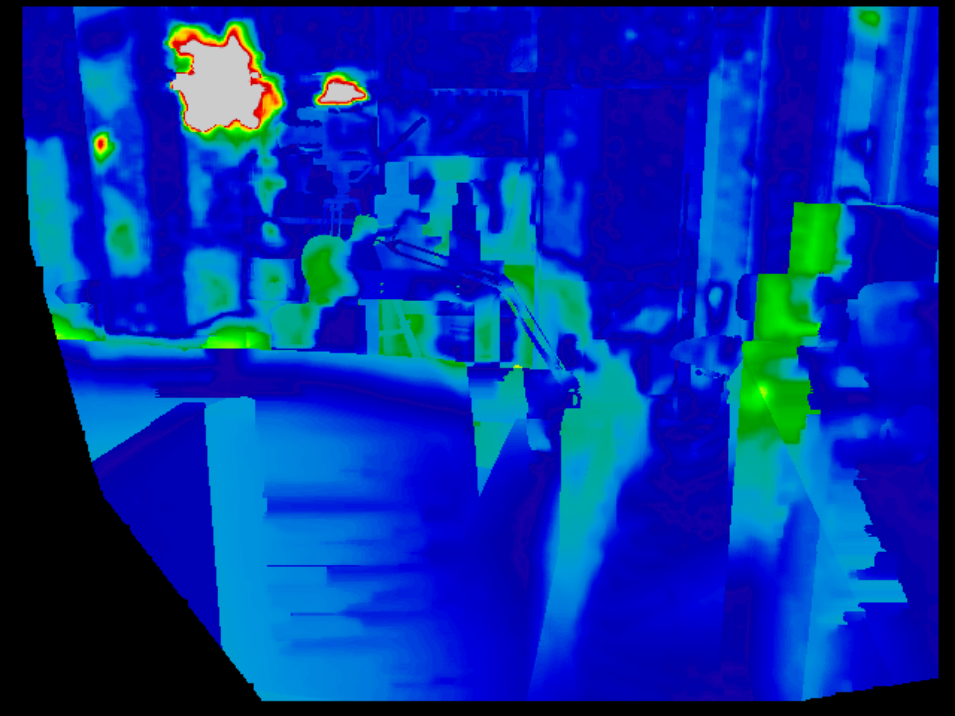
\includegraphics[width=0.2\columnwidth]{./images/tsukuba_frame1314_libelas_error_high6.png}%
%			\label{tsukuba_frame1314_libelas_error}}
%        \hfil
%		\subfloat[Dense S-PTAM dmap]{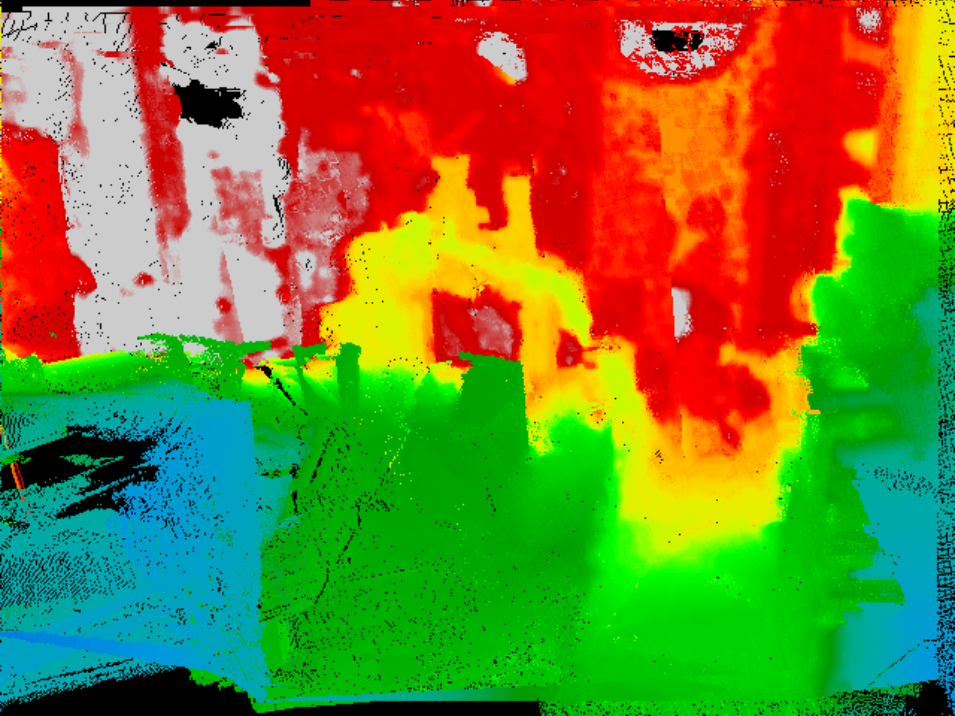
\includegraphics[width=0.2\columnwidth]{./images/tsukuba_frame1314_dense_high6.png}%
%			\label{tsukuba_frame1314_dense}}
%        \hfil
%		\subfloat[Dense S-PTAM dmap error]{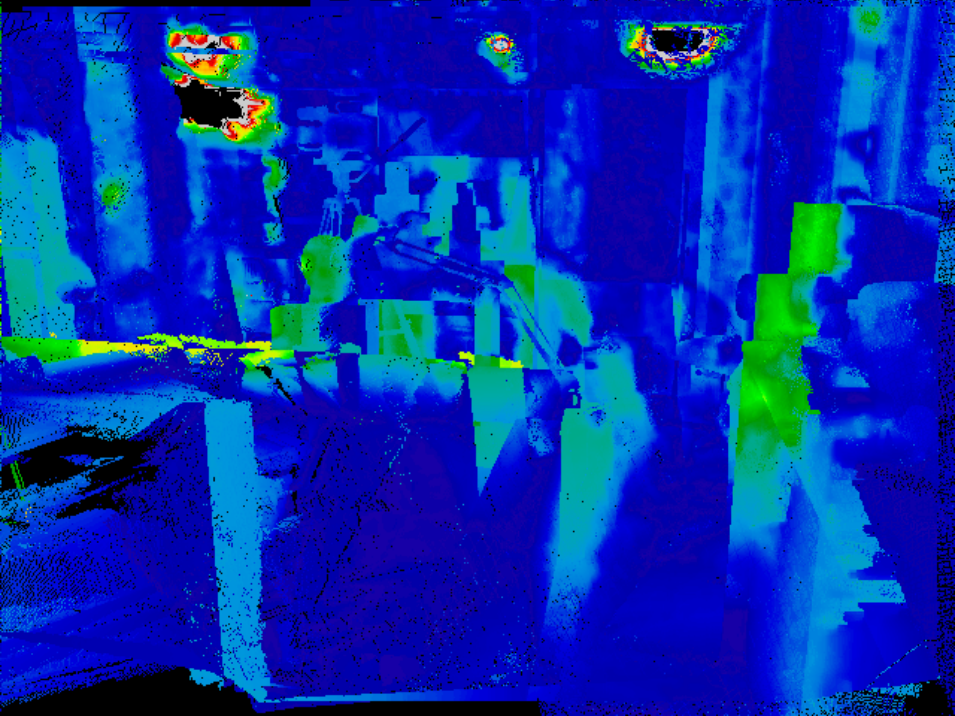
\includegraphics[width=0.2\columnwidth]{./images/tsukuba_frame1314_error_high6.png}%
%			\label{tsukuba_frame1314_error}}
%		\\
%		\subfloat[]{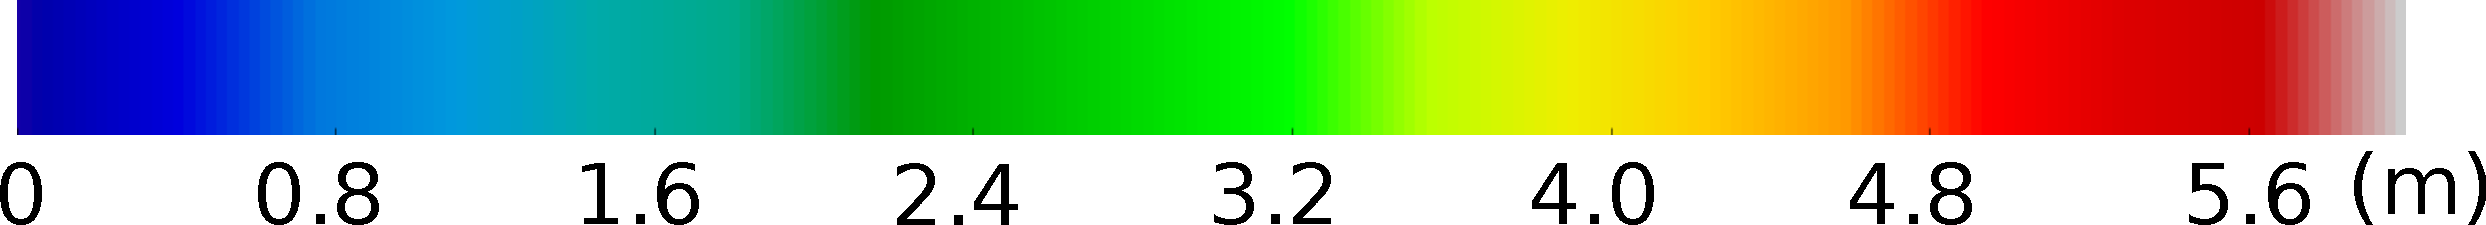
\includegraphics[width=0.4\columnwidth]{./images/high6_bar.pdf}%
%			\label{tsukuba_frame1314_bar}}
%		\caption{Comparison: LIBELAS, DS-PTAM dmaps against GT (Tsukuba)}
%		\label{fig:tsukuba_frame1314}
%	\end{figure}
%\end{frame}

%\begin{frame}
%	\frametitle{KITTI error}
%	\begin{figure}[!htb]
%		\centering
%		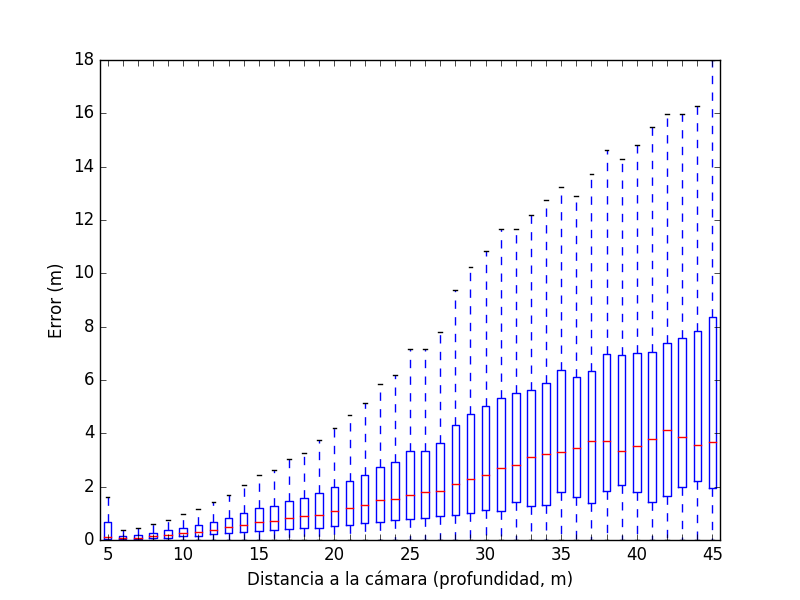
\includegraphics[width=0.33\columnwidth]{images/kitti06_libelas_boxplot}
%		\caption{LIBELAS errors (depth vs errors) on KITTI sequence 06.}
%		\label{fig:kitti06_libelas_boxplot}
%	\end{figure}
%	
%	\begin{figure}[!htb]
%		\centering
%		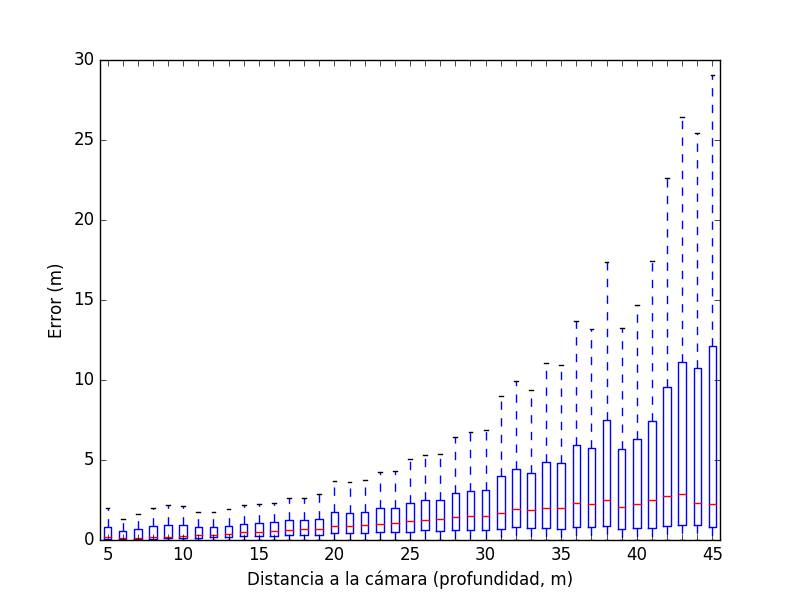
\includegraphics[width=0.33\columnwidth]{images/kitti06_dense_boxplot}
%		\caption{Dense S-PTAM errors (depth vs errors) on KITTI sequence 06.}
%		\label{fig:kitti06_dense_boxplot}
%	\end{figure}
%\end{frame}

\begin{frame}
	\frametitle{KITTI: error de mediana}
	\begin{figure}[!htb]
		\centering
		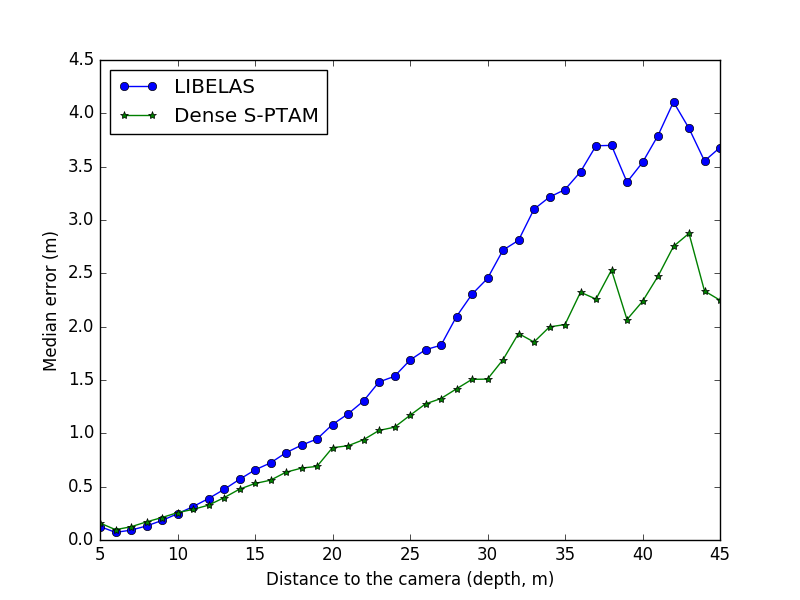
\includegraphics[width=0.8\columnwidth]{images/medians_comparison_kitti}
%		\caption{Median error comparison between LIBELAS and dense (depth vs errors) on KITTI sequence 06.}
		\caption{Comparación del error de mediana entre las reconstruccones obtenidas por LIBELAS y Dense en la secuencia de KITTI 06.}
		\label{fig:median_comparison_kitti}
	\end{figure}
\end{frame}

%\begin{frame}
%	\frametitle{Tsukuba error}
%	\begin{figure}[!htb]
%		\centering
%		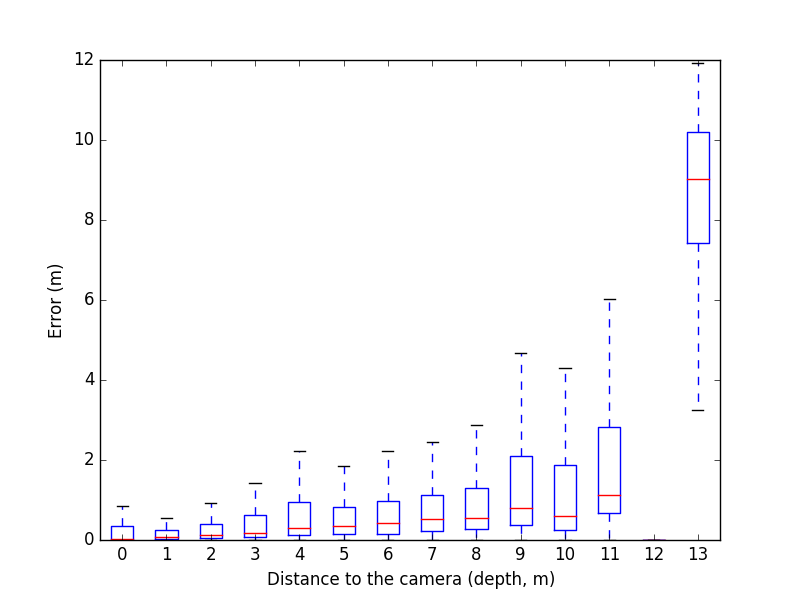
\includegraphics[width=0.33\columnwidth]{images/tsukuba_libelas_boxplot}
%		%\caption{LIBELAS raw reconstruction errors (depth vs errors) in dataset Tsukuba.}
%		\label{fig:tsukuba_libelas_boxplot}
%	\end{figure}
%	\begin{figure}[!htb]
%		\centering
%		\includegraphics[width=0.33\columnwidth]{images/tsukuba_dense_boxplot}
%		%\caption{Errors (depth vs errors) in dataset Tsukuba.}
%		\label{fig:tsukuba_dense_boxplot}
%	\end{figure}
%\end{frame}

\begin{frame}
	\frametitle{Tsukuba: error de mediana}
	\begin{figure}[!htb]
		\centering
		\includegraphics[width=0.8\columnwidth]{images/medians_comparison_tsukuba}
		%\caption{Median error comparison between LIBELAS and Dense S-PTAM (depth vs errors) on Tsukuba sequence.}
		\caption{Comparación del error de mediana entre las reconstruccones obtenidas por LIBELAS y Dense en la secuencia de Tsukuba.}
		\label{fig:median_comparison_tsukuba}
	\end{figure}
\end{frame}

\begin{frame}
	\frametitle{Cantidad de puntos}
	\begin{figure}[!htb]
		\centering
		\subfloat[KITTI]{\includegraphics[width=0.45\columnwidth]{./images/points_kitti06}%
			\label{tsukuba_frame1314_rgb}}
		\hfil
		\subfloat[Tsukuba]{\includegraphics[width=0.45\columnwidth]{./images/points_tsukuba}%
			\label{tsukuba_frame1314_gt}}
	\end{figure}
\end{frame}
	
%\begin{frame}
%	\frametitle{Cantidad de puntos}
%	\begin{figure}[!htb]
%		\centering
%		\includegraphics[width=\columnwidth]{images/points_kitti06}
%		\caption{Total amount of points during the Dense S-PTAM execution (generated, discarded, present on final reconstruction---hypotheses (saw one time) and validated (fused multiple times)---, and number of fusions) on KITTI 06 sequence.}
%		\label{fig:points_kitti}
%	\end{figure}
%\end{frame}
%
%\begin{frame}
%	\frametitle{Cantidad de puntos}
%\begin{figure}[!htb]
%	\centering
%	\includegraphics[width=\columnwidth]{images/points_tsukuba}
%	\caption{Total amount of points during the Dense S-PTAM execution (generated, discarded, present on final reconstruction---hypotheses (saw one time) and validated (fused multiple times)---, and number of fusions) on Tsukuba sequence.}
%	\label{fig:points_tsukuba}
%\end{figure}
%\end{frame}

\begin{frame}
	\frametitle{Análisis de tiempos}
	\begin{table}[!htb]
		\centering
		\small
		\begin{tabular}{cccc}
			\toprule
			Sequence & Disparity (ms) & Map Fusion (ms) & Map Refinement (ms) \\
			\midrule
			KITTI 06 & 202.66 & 124.76 & 8.00 \\
			Tsukuba & 98.88 & 127.10 & 1.66 \\
			\bottomrule
		\end{tabular}
		%\caption{Average computation times (in ms) for each of the main steps of our algorithm.}
		\caption{Promedio de los tiempos requeridos (en ms) por cada uno de los principales pasos Dense.}
		\label{table:table_times}
	\end{table}
\end{frame}

\begin{frame}
	\frametitle{S-PTAM Denso!}
	\centering
	
	\inlineMovie[loop&autostart&start=5]{./videos/sptam_dense_online.mp4}{./images/kitti_3d_2}{width=\columnwidth}
\end{frame}

\begin{frame}
	\frametitle{S-PTAM Denso!}
	\centering
	
	\inlineMovie[loop&autostart&start=5]{./videos/sptam_dense_offline.mp4}{./images/kitti_3d_2}{width=\columnwidth}
\end{frame}
